\documentclass{article}
\usepackage[english]{babel}
\usepackage{amsmath,amssymb,graphicx,mathrsfs,xcolor,latexsym,theorem,natbib}

%%%%%%%%%% Start TeXmacs macros
\newcommand{\cdummy}{\cdot}
\newcommand{\mathd}{\mathrm{d}}
\newcommand{\tmaffiliation}[1]{\\ #1}
\newcommand{\tmcolor}[2]{{\color{#1}{#2}}}
\newcommand{\tmem}[1]{{\em #1\/}}
\newcommand{\tmtextbf}[1]{\text{{\bfseries{#1}}}}
\newcommand{\tmtextit}[1]{\text{{\itshape{#1}}}}
\newcommand{\tmtextsc}[1]{\text{{\scshape{#1}}}}
\newenvironment{proof}{\noindent\textbf{Proof\ }}{\hspace*{\fill}$\Box$\medskip}
{\theorembodyfont{\rmfamily}\newtheorem{example}{Example}}
\newtheorem{proposition}{Proposition}
{\theorembodyfont{\rmfamily}\newtheorem{remark}{Remark}}
\newtheorem{theorem}{Theorem}
%%%%%%%%%% End TeXmacs macros

\newtheorem{assumption}{assumption}
\newcommand{\R}{\mathbb{R}}
\newcommand{\Q}{\ensuremath{\mathbb{Q}}}
\newcommand{\N}{\mathbb{N}}
\newcommand{\Z}{\mathbb{Z}}
\newcommand{\dif}{ \langle \mathd \rangle }
\newcommand{\C}{\mathbb{C}}
\newcommand{\toni}[1]{\tmcolor{blue}{\tmtextbf{Toni:} #1}}
\newcommand{\filip}[1]{{\color[HTML]{228B22}\tmtextbf{Filip:} #1}}
\newcommand{\rev}[1]{\tmcolor{black}{#1}}

\begin{document}

\title{{\Large \tmtextbf{Orthonormal Expansions for Translation-Invariant
Kernels}}}

\author{
  Filip TronarpToni Karvonen
  \tmaffiliation{Centre for Mathematical Sciences, Lund University, Sweden}
  \tmaffiliation{Department of Mathematics and Statistics, University of
  Helsinki, Finland \ September 20, 2024}
}

\maketitle

\begin{abstract}
  {\noindent}We present a general Fourier analytic technique for constructing
  orthonormal basis expansions of translation-invariant kernels from
  orthonormal bases of $\mathscr{L}_2 (\mathbb{R})$. This allows us to derive
  explicit expansions on the real line for (i) Mat{\'e}rn kernels of all
  half-integer orders in terms of associated Laguerre functions, (ii) the
  Cauchy kernel in terms of rational functions, and (iii) the Gaussian kernel
  in terms of Hermite functions.\\
  \\
  \tmtextbf{Keywords:} positive-definite kernels, radial basis functions,
  orthonormal expansions, orthogonal polynomials\\
  \\
  \tmtextbf{MSC2020:} 65D12, 46E22, 33C45, 60G10
\end{abstract}

\section{Introduction}\label{sec:introduction}

Let $\Omega$ be a vector space. A symmetric positive-semidefinite kernel $r :
\Omega \times \Omega \to \R$ is {\tmem{translation-invariant}} if $r (t, u) =
\Phi (t - u)$ for some $\Phi : \Omega \to \R$ and all $t, u \in \Omega$.
Translation-invariant kernels, also known as {\tmem{stationary}} or
{\tmem{shift-invariant}} kernels, are a mainstay of radial basis function
interpolation~{\cite{Wendland2005}} and Gaussian process modelling as used in,
for example, spatial statistics~{\cite{Stein1999}} and machine
learning~{\cite{RasmussenWilliams2006}}. Each positive-semidefinite kernel
induces a unique reproducing kernel Hilbert space (RKHS), $\mathscr{H}_r
(\Omega)$, which is equipped with an inner product $\langle \cdummy, \cdummy
\rangle_r$ and the associated norm
$\normstar{0}{\cdot}_r$~{\rev{{\citep{[}}Section~2.2]Paulsen2016}}.
Practically every commonly used kernel induces an infinite-dimensional RKHS
that is separable (see~{\cite{OwhadiScovel2017}} for a short review on
separability of RKHSs), which means that $\mathscr{H}_r (\Omega)$ has an
orthonormal basis $\{\psi_m \}_{m \in I}$ for some countably infinite index
set $I$ (e.g., $I = \N$) and that the kernel admits the pointwise convergent
orthonormal expansion
\begin{equation}
  \label{eq:kernel-expansion-intro} r (t, u) = \sum_{m \in I} \psi_m^{\ast}
  (t) \psi_m (u)  \quad \text{for all } \quad t, u \in \Omega,
\end{equation}
{\rev{where $z^{\ast}$ denotes the complex conjugate of $z \in \C$.}} If
$\Omega$ is a compact subset {\rev{of the Euclidean space}} $\R^d$ and $r$ is
continuous, the expansion~\eqref{eq:kernel-expansion-intro} converges
uniformly~{\citep{Paulsen2016}}. Expansions of the
form~\eqref{eq:kernel-expansion-intro} are often needed to develop reduced
rank methods of sub-cubic computational
complexity~{\cite{RahimiRecht2007,SolinSarkka2020}}, to improve numerical
stability~{\cite{FasshauerMcCourt2012}}, and for various theoretical
purposes~{\cite[e.g.,]{[}}]Karvonen2022, Steinwart2019.

However, few orthonormal expansions appear to have been constructed for
translation-invariant kernels. To the best of our knowledge, the
Mat{\'e}rn-$\frac{1}{2}$ kernel $r (t, u) = \exp (- \lambda \absstar{0}{t -
u})$ and the Gaussian kernel $r (t, u) = \exp (- \frac{1}{2} \lambda^2 (t -
u)^2)$ on subsets of $\R$ are the only commonly used translation-invariant
kernels for which orthonormal expansions have been found. For various
expansions of the Mat{\'e}rn-$\frac{1}{2}$ kernel, see Section~4 in
{\cite{Hawkins1989}}, Section~3.4.1 in {\cite{VanTrees2001}}, Example~4.1 in
{\cite{Xiu2010}}, and Example~2.5 and Appendix~A.2 in
{\cite{FasshauerMcCourt2015}}. For the Gaussian kernel both a simple
non-Mercer expansion based on a Taylor expansion of the exponential
function~{\cite[e.g.,]{[}}]Minh2010 and a class of Mercer
expansions~{\cite[Section~12.2.1]{FasshauerMcCourt2015}}, which appear to have
originated in~{\cite[Section~4]{Zhu1998}}, are available. A large collection
of expansions for kernels which are not translation-invariant can be found
in~{\cite[Appendix~A]{FasshauerMcCourt2015}}. In this article we describe a
general and conceptually simple Fourier analytic technique, contained in
Theorem~\ref{thm:main-theorem}, for constructing orthonormal bases for
translation-invariant kernels on $\R$ out of orthonormal bases of
$\mathscr{L}_2 (\R)$. We then use this technique to compute orthonormal
expansions for three commonly used classes of kernels.

Ours is what one could call a {\tmem{kernel-centric}} approach. That is, our
starting point is a kernel that has, in some sense, desirable or intuitive
properties and our goal is to {\rev{find}} its orthonormal expansion. The
{\tmem{space-centric}} approach is to start with a Hilbert space or its
orthonormal basis, show that this space is an RKHS, and construct its
reproducing kernel via~\eqref{eq:kernel-expansion-intro}; under fortuitous
circumstances the kernel is available in closed form. A prime example of this
approach is how Korobov spaces and their kernels, which can be expressed in
terms of Bernoulli polynomials, are used in the quasi-Monte Carlo
literature~{\cite[e.g.,]{[}}Section~5.8]DickKuoSloan2013. Other examples
include Hardy spaces~{\cite[Section~1.4.2]{Paulsen2016}}, power series
kernels~{\cite{Zwickngaslc2009}}, and Hermite
spaces~{\cite{IrrgeherLeobacher2015}}. Our technique to construct orthonormal
bases is similar to the method in~{\cite{NovakUllrich2018}}, where the goal is
however to find a closed form expression for the reproducing kernel of a
Hilbert space.

\subsection{Construction of orthonormal bases}

{\rev{Let $\absstar{0}{z}$ denote the modulus of $z \in \C$ and recall that
$z^{\ast}$ is the complex conjugate.}} The spaces $\mathscr{L}_2 (\R)$ and
$\mathscr{L}_2 (\R, 1 / 2 \pi)$ consist of all square-integrable functions $f
: \R \to \C$ and are equipped with the inner products
\[ \langle f, g \rangle_{\mathscr{L}_2 (\R)} = \int_{- \infty}^{\infty}
   f^{\ast} \hspace{-0.17em} (t) g (t) \dif t \quad \text{and } \quad \langle
   f, g \rangle_{\mathscr{L}_2 (\R, 1 / 2 \pi)} = \frac{1}{2 \pi}  \int_{-
   \infty}^{\infty} f^{\ast} \hspace{-0.17em} (t) g (t) \dif t. \]
The Fourier transform and the corresponding inverse transform for any
integrable or square-integrable function $f$ are defined as
\[ \hat{f} (\omega) = \int_{- \infty}^{\infty} f (t) e^{- i \omega t} \dif t
   \quad \text{and } \quad f (t) = \frac{1}{2 \pi}  \int_{- \infty}^{\infty}
   \hat{f} (\omega) e^{i \omega t} \dif \omega . \]
The Fourier transform defines an isometry from $\mathscr{L}_2 (\mathbb{R})$ to
$\mathscr{L}_2 (\mathbb{R}, 1 / 2 \pi)$ via the Plancherel theorem
\[ \int_{- \infty}^{\infty} f^{\ast} \hspace{-0.17em} (t) g (t) \dif t =
   \frac{1}{2 \pi}  \int_{- \infty}^{\infty} \hat{f}^{\ast} \hspace{-0.17em}
   (\omega)  \hat{g} (\omega) \dif \omega . \]
The functions $f$ and $\hat{f}$ are referred to as time domain and Fourier
domain representations, respectively. Our $\mathscr{H}_r (\R)$-orthonormal
expansions are derived from the following rather straight-forward theorem. Let
$I$ be a countably infinite index set, typically either $\N$ or $\Z$.

\begin{theorem}
  [Construction of orthonormal bases]\label{thm:main-theorem}{\rev{Suppose
  that $r (t, u) = \Phi (t - u)$ is a translation-invariant symmetric
  positive-definite kernel with $\Phi \in C (\R) \cap \mathscr{L}_1 (\R)$. Let
  $\{\varphi_m \}_{m \in I}$ be an orthonormal basis of $\mathscr{L}_2 (\R)$
  and $h$ a function such that $\absstar{0}{\hat{h} (\omega)} = \hat{\Phi}
  (\omega)^{1 / 2}$.}} Then the functions
  \[ \psi_m (t) = \int_{- \infty}^{\infty} h (t - \tau) \varphi_m (\tau) \dif
     \tau \quad \text{with Fourier transforms } \quad \hat{\psi}_m (\omega) =
     \hat{h} (\omega)  \hat{\varphi}_m (\omega) \]
  for $m \in I$ form an orthonormal basis of $\mathscr{H}_r (\R)$ and the
  kernel $r$ has the pointwise convergent expansion
  \begin{equation}
    \label{eq:main-theorem-r-expansion} r (t, u) = \sum_{m \in I}
    \psi_m^{\ast} (t) \psi_m (u)  \quad \text{for all } \quad t, u \in \R .
  \end{equation}
\end{theorem}

\begin{proof}
  {\rev{That $r$ is symmetric positive-definite implies that $\hat{\Phi}$ is
  real-valued and positive~{\cite[Theorem~6.11]{Wendland2005}}.}} For a
  function $h$ such that $\absstar{0}{\hat{h} (\omega)} = \hat{\Phi}
  (\omega)^{1 / 2} > 0$ for all $\omega \in \R$ we define a convolution
  operator $\mathcal{H}: \mathscr{L}_2 (\R) \to \mathscr{L}_2 (\R)$ via
  \[ (\mathcal{H}f) (t) = \int_{- \infty}^{\infty} h (t - \tau) f (\tau) \dif
     \tau \quad \text{for all } \quad t \in \R . \]
  Note that the convolution theorem yields $\widehat{\mathcal{H}f} (\omega) =
  \hat{h} (\omega)  \hat{f} (\omega)$. By the standard characterisation
  (see~{\cite{KimeldorfWahba1970}} or~{\cite[Theorem~10.12]{Wendland2005}}) of
  the RKHS of a translation-invariant kernel,
  \begin{equation}
    \label{eq:RKHS-fourier} \langle f, g \rangle_r = \frac{1}{2 \pi}  \int_{-
    \infty}^{\infty} \frac{\hat{f}^{\ast} \hspace{-0.17em} (\omega)  \hat{g}
    (\omega)}{\hat{\Phi} (\omega)} \dif \omega \quad \text{for any } \quad f,
    g \in \mathscr{H}_r (\R) .
  \end{equation}
  For any $f, g \in \mathscr{L}_2 (\R)$ the convolution theorem and Plancherel
  theorem thus give
  \[ \langle \mathcal{H}f, \mathcal{H}g \rangle_r = \frac{1}{2 \pi}  \int_{-
     \infty}^{\infty} \frac{\absstar{0}{\hat{h} (\omega)}^2 \hat{f}^{\ast}
     \hspace{-0.17em} (\omega)  \hat{g} (\omega)}{\hat{\Phi} (\omega)} \dif
     \omega = \frac{1}{2 \pi}  \int_{- \infty}^{\infty} \hat{f}^{\ast}
     \hspace{-0.17em} (\omega)  \hat{g} (\omega) \dif \omega = \langle f, g
     \rangle_{\mathscr{L}_2 (\R)}, \]
  which shows that $\mathcal{H}$ is an isometry from $\mathscr{L}_2 (\R)$ to
  $\mathscr{H}_r (\R)$. It follows from~\eqref{eq:RKHS-fourier} that the
  inverse Fourier transform
  \[ (\mathcal{H}^{- 1} f) (t) = \frac{1}{2 \pi}  \int_{- \infty}^{\infty}
     \frac{\hat{f} (\omega)}{\hat{h} (\omega)} e^{i \omega t} \dif \omega
     \quad \text{for all } \quad t \in \R \]
  defines the inverse of $\mathcal{H}$. Therefore $\mathcal{H}$ is an
  isometric isomorphism and thus maps every orthonormal basis of
  $\mathscr{L}_2 (\R)$ to an orthonormal basis of $\mathscr{H}_r
  (\R)$~{\cite[Section~2.6]{Higgins1977}}. {\rev{The kernel has a pointwise
  convergent expansion of the form~\eqref{eq:main-theorem-r-expansion} for
  every orthonormal basis of $\mathscr{H}_r (\R)$~{\citep{Paulsen2016}}.}}
\end{proof}

To obtain the basis functions $\psi_m$ in time domain using 
Theorem~\ref{thm:main-theorem} one has to either compute the convolution
$\int_{- \infty}^{\infty} h (t - \tau) \rev{\varphi_m (\tau)} \dif \tau$ or
the inverse Fourier transform of $\hat{h} (\omega)  \hat{\varphi}_m (\omega)$.
It is therefore necessary to select a basis of $\mathscr{L}_2 (\R)$ for which
either of these operations can be done in closed form. We use 
Theorem~\ref{thm:main-theorem} to derive orthonormal expansions for (i)
Mat{\'e}rn kernels for all half-integer orders, (ii) the Cauchy kernel (i.e.,
rational quadratic kernel~{\cite[Equation~(4.19)]{RasmussenWilliams2006}} with
$\alpha = 1$), and (iii) the Gaussian kernel. The expansions are summarised in
Section~\ref{sec:summary}. {\rev{All expansions appearing in this article
converge pointwise.}}

\subsection{On Mercer expansions}

Let $\Omega$ be a subset of $\R^d$ and $w : \Omega \to [0, \infty)$ a weight
function. The Hilbert space $\mathscr{L}_2 (\Omega, w)$ is equipped with the
inner product
\[ \langle f, g \rangle_{\mathscr{L}_2 (\Omega, w)} = \int_{\Omega} f^{\ast}
   \hspace{-0.17em} (t) g (t) w (t) \dif t \]
and consists of all functions $f : \R \to \C$ for which the corresponding norm
is finite. Suppose that the kernel $r$ is continuous and define the integral
operator
\begin{equation}
  \label{eq:mercer-integral-operator} \mathcal{T}_{r, w} f = \int_{-
  \infty}^{\infty} r (\cdummy, u) f (u) w (u) \dif u.
\end{equation}
Under certain assumptions, Mercer's theorem~{\cite{SteinwartScovel2012}}
states that (i) $\mathcal{T}_{r, w}$ has continuous eigenfunctions $\{
\rev{\vartheta}_m \}_{m = 0}^{\infty}$ and corresponding positive
non-increasing eigenvalues $\{\mu_m \}_{m = 0}^{\infty}$ which tend to zero,
(ii) $\{ \rev{\vartheta}_m \}_{m = 0}^{\infty}$ are an orthonormal basis of
$\mathscr{L}_2 (\Omega, w)$, and (iii) $\{ \sqrt{\smash{[} b] \mu_m}
\rev{\vartheta}_m \}_{m = 0}^{\infty}$ is an orthonormal basis of
$\mathscr{H}_r (\Omega)$. Consequently, the kernel has the pointwise
convergent {\tmem{Mercer expansion}}
\begin{equation}
  \label{eq:kernel-expansion-mercer} r (t, u) = \sum_{m = 0}^{\infty} \mu_m
  \rev{\vartheta}_m^{\ast} (t) \rev{\vartheta}_m (u)  \quad \text{for all }
  \quad t, u \in \Omega .
\end{equation}
While Mercer's theorem and the eigenvalues of $\mathcal{T}_{r, w}$ constitute
a powerful tool for understanding topics such as optimal approximation in
$\mathscr{L}_2 (\Omega, w)$-norm
(e.g.,~{\cite[Corollary~4.12]{NovakWozniakowski2008}}
and~{\cite[Section~2.4]{FasshauerHickernell2012}}) and improved approximation
orders in subsets of $\mathscr{H}_r
(\Omega)$~{\cite[Section~11.5]{Wendland2005}}, both in theoretical research
and practical applications there is often no reason to prefer a Mercer
expansion~\eqref{eq:kernel-expansion-mercer} over a generic RKHS-orthonormal
expansion~\eqref{eq:kernel-expansion-intro}. For example, the
Karhunen--Lo{\`e}ve theorem is merely a special case of a more general result
that a Gaussian process with covariance kernel~$r$ can be expanded in terms of
any orthonormal basis of $\mathscr{H}_r
(\Omega)$~{\cite[Chapter~III]{Adler1990}}. When an expansion is being sought
{\rev{solely for}} computational reasons, it does not matter whether or not
this expansion is Mercer.

Constructing a Mercer expansion by first identifying a convenient weight and
then finding the eigendecomposition of the integral
operator~\eqref{eq:mercer-integral-operator} can be rather involved, which is
illustrated by the construction in~{\cite[Example~2.5]{FasshauerMcCourt2015}}
for the Mat{\'e}rn-$\frac{1}{2}$ kernel. What makes 
Theorem~\ref{thm:main-theorem} convenient is therefore that it does
{\tmem{not}} require that the expansion be Mercer for some weight. However,
identifying a weight $w$ for which the basis function $\psi_m$ constructed via
Theorem~\ref{thm:main-theorem} are $\mathscr{L}_2 (\R, w)$-orthogonal shows
that the expansion is Mercer because the $\mathscr{L}_2 (\R, w)$-normalised
versions of $\psi_m$ are the eigenfunctions of $\mathcal{T}_{r, w}$. It turns
out that our expansion for the Gaussian kernel is Mercer and the ones for
Mat{\'e}rn kernels are ``almost'' Mercer, in that all but finitely many basis
functions are orthogonal in $\mathscr{L}_2 (\R, w)$ for a certain weight.

\section{Summary of expansions}\label{sec:summary}

This section summarises the expansions that we derive using 
Theorem~\ref{thm:main-theorem}. Each expansion converges pointwise for all $t,
u \in \R$. All expansions are for kernels with unit scaling. Expansions of
arbitrary scalings, $\lambda$, may be obtained by considering the kernel $r
(\lambda t, \lambda u)$, for which the corresponding basis functions are
$\psi_m  (\lambda t)$.

\subsection{Mat{\'e}rn kernels}

Expansions for Mat{\'e}rn kernels are derived in  Section~\ref{sec:matern}. A
Mat{\'e}rn kernel of order $\alpha > 0$ is
\begin{equation}
  \label{eq:matern-kernel-intro} r_{\alpha} (t, u) = \frac{2^{1 -
  \alpha}}{\Gamma (\alpha)} (\absstar{0}{t - u})^{\alpha} \mathrm{K}_{\alpha}
  (\absstar{0}{t - u}),
\end{equation}
where $\Gamma$ is the Gamma function and $\mathrm{K}_{\alpha}$ the modified
Bessel function of the second kind of order~$\alpha$. Let
$\mathrm{L}_m^{(\eta)}$ denote the $m$th associated Laguerre polynomial of
index $\eta$, defined in~\eqref{eq:associated-laguerre}, and let $\{\varphi_m
\}_{m \in \Z}$ be the Laguerre functions
\[ \varphi_m (t) = \sqrt{2} \hspace{0.17em} \mathrm{L}_m (2 t) e^{- t} 
   \textbf{1}_{[0, \infty)} (t)  \quad \text{and } \quad \varphi_{- m - 1} (t)
   = - \sqrt{2} \hspace{0.17em} \mathrm{L}_m (- 2 t) e^t  \textbf{1}_{(-
   \infty, 0)} (t) \]
for $m \in \N_0$, where $\mathrm{L}_m = \mathrm{L}_m^{(0)}$ and $\textbf{1}_A$
denotes the indicator function of a set $A$. Consider half-integer order
$\alpha = \nu + 1 / 2$ for $\nu \in \N_0$. Then the Mat{\'e}rn-Laguerre
functions

\begin{align*}
  \psi^+_{m, \nu} (t) & = \frac{\nu !}{(2 \nu) !}  \frac{m!}{(m + \nu + 1) !} 
  (2 t)^{\nu + 1} \mathrm{L}_m^{(\nu + 1)} (2 t) e^{- t}  \textbf{1}_{[0,
  \infty)} (t) &  & \text{for } \quad m \in \mathbb{N}_0\\
  \psi^-_{m, \nu} (t) & = (- 1)^{\nu} \psi^+_{m, \nu}  (- t) &  & \text{for }
  \quad m \in \mathbb{N}_0,\\
  \psi^0_{m, \nu} (t) & = \frac{1}{\sqrt{\smash{[} b] 2}}  \frac{\nu
  !}{\sqrt{\smash{[} b] (2 \nu) !}}  \sum_{k = 0}^{\nu + 1} \binom{\nu + 1}{k}
  (- 1)^k \varphi_{m + k - \nu - 1} (t) &  & \text{for } m = 0, \ldots, \nu
\end{align*}

form an orthonormal basis of the RKHS and
\[ r_{\nu + 1 / 2,} (t, u) = \sum_{m = 0}^{\nu} \psi^0_{m, \nu} (t) \psi^0_{m,
   \nu} (u) + \sum_{m = 0}^{\infty} \psi^-_{m, \nu} (t) \psi^-_{m, \nu} (u) +
   \sum_{m = 0}^{\infty} \psi^+_{m, \nu} (t) \psi^+_{m, \nu} (u) \]
for all $t, u \in \R$. The basis functions $\smash{[} b] \psi_{m, \nu}^-$ and
$\smash{[} b] \psi_{m, \nu}^+$ are orthogonal in $\mathscr{L}_2 (\R, w_{\nu})$
for the weight function $\smash{[} b] w_{\nu} (t) = 2 / \abs{2 t}^{\nu + 1}$.

\subsection{Cauchy kernel}

Expansions for the Cauchy kernel are derived in  Section~\ref{sec:cauchy}. The
Cauchy kernel is
\[ r (t, u) = \frac{1}{1 + (t - u)^2} . \]
Both the complex-valued Cauchy--Laguerre functions
\[ \psi_m (t) = - \frac{1}{\sqrt{2}}  \frac{(it)^m}{(it - 1)^{m + 1}}  \quad
   \text{and } \quad \psi_{- m - 1} (t) = - \frac{1}{\sqrt{2}} 
   \frac{(it)^m}{(it + 1)^{m + 1}} \]
for $m \in \N_0$ and the {\rev{real-valued Cauchy--Laguerre functions}}
\[ \alpha_m (t) = \frac{1}{\sqrt{2}}  (\psi_m (t) + \psi_m^{\ast} (t))  \quad
   \text{and} \quad \beta_m (t) = \frac{1}{\sqrt{2}}  (\psi_m (t) -
   \psi_m^{\ast} (t)) \]
for $m \in \N_0$ form orthonormal bases of the RKHS. Therefore, the Cauchy
kernel has the expansions
\[ r (t, u) = \sum_{m = - \infty}^{\infty} \psi_m^{\ast} (t) \psi_m (u) =
   \sum_{m = 0}^{\infty} \alpha_m (t) \alpha_m (u) + \sum_{m = 0}^{\infty}
   \beta_m (t) \beta_m (u) \]
for all $t, u \in \R$. Expressions of $\alpha_m$ and $\beta_m$ in terms of
real parameters are given in \eqref{eq:real_cauchy_laguerre_explicit}.

\subsection{Gaussian kernel}

Expansions for the Gaussian kernel are derived in  Section~\ref{sec:gaussian}.
The Gaussian kernel is
\[ r (t, u) = \exp \left( \hspace{-0.17em} - \frac{1}{2} (t - u)^2 \right) .
\]
The functions
\begin{equation}
  \label{eq:gaussian-basis-intro} \psi_m (t) = \left( \frac{2 \sqrt{2}}{3}
  \right)^{1 / 2} \sqrt{\frac{1}{6^m m!}} e^{- t^2 / 3} \mathrm{H}_m \left(
  \frac{2 t}{\sqrt{3}} \right)  \quad \text{for } \quad m \in \N_0
\end{equation}
form an orthonormal basis of the RKHS and the kernel has the expansion
\[ r (t, u) = \sum_{m = 0}^{\infty} \psi_m (t) \psi_m (u) \]
for all $t, u \in \R$. This expansion is a special case of the well-known
Mercer expansion of the Gaussian
kernel~{\cite[Section~12.2.1]{FasshauerMcCourt2015}}. The basis
functions~\eqref{eq:gaussian-basis-intro} are orthogonal in $\mathscr{L}_2
(\R, w_{\alpha})$ for the weight function $w_{\alpha} (t) = \alpha \pi^{- 1 /
2} e^{- \alpha^2 t^2}$ with $\alpha = \sqrt{\smash{[} b] 2 / 3}$.

\section{Expansions of Mat{\'e}rn kernels}\label{sec:matern}

The Mat{\'e}rn kernel of order $\alpha > 0$ in~\eqref{eq:matern-kernel-intro}
can be written as
\[ r_{\alpha} (t, u) = \frac{2^{1 - 2 \alpha}}{\Gamma (\alpha)} (2 \abs{t -
   u})^{\alpha} \mathrm{K}_{\alpha} (\absstar{0}{t - u}), \]
and its Fourier transform is~{\rev{{\citep{[}}Theorem~6.13]Wendland2005}}
\[ \hat{\Phi}_{\alpha} (\omega) = 2^{1 - 2 \alpha}  \sqrt{\pi} 
   \hspace{0.17em} \frac{\Gamma (\alpha + 1 / 2)}{\Gamma (\alpha)}  \frac{2^{2
   \alpha}}{(\omega^2 + 1)^{\alpha + 1 / 2}} . \]
From now on we assume that the kernel is of half-integer order: $\alpha = \nu
+ 1 / 2$ for $\nu \in \N_0$. Then the Fourier transform simplifies to
\[ \hat{\Phi}_{\nu + 1 / 2} (\omega) = \frac{(\nu !)^2}{(2 \nu) !}  \frac{2^{2
   \nu + 1}}{(\omega^2 + 1)^{\nu + 1}}, \]
and a non-symmetric square-root, in the sense that $\absstar{0}{\hat{h}_{\nu +
1 / 2} (\omega)}^2 = \hat{\Phi}_{\nu + 1 / 2} (\omega)$, is given by
\begin{equation}
  \label{eq:h-hat-matern} \hat{h}_{\nu + 1 / 2} (\omega) = \frac{\nu
  !}{\sqrt{\smash{[} b] (2 \nu) !}}  \frac{2^{\nu + 1 / 2}}{(i \omega +
  1)^{\nu + 1}} .
\end{equation}
The corresponding time domain function is~{\cite[Section~1.03]{Wiener1949}}
\begin{equation}
  \label{eq:h-matern} h_{\nu + 1 / 2} (t) = 2^{\nu + 1 / 2}  \frac{\nu
  !}{\sqrt{\smash{[} b] (2 \nu) !}}  \frac{t^{\nu}}{\nu !} e^{- t} 
  \textbf{1}_{[0, \infty)} (t) .
\end{equation}
{\rev{Note that}} this function vanishes on the negative real line.

\subsection{Laguerre functions}\label{sec:laguerre-functions}

The following material is mostly based on Section~2.6.4
in~{\cite{Higgins1977}} and Section~1.03 in~{\cite{Wiener1949}}. To derive an
orthonormal expansion for the Mat{\'e}rn kernel we use the so-called
{\tmem{Laguerre functions}} $\varphi_m$ whose Fourier transforms are given by
\begin{equation}
  \label{eq:laguerre-func-ft} \hat{\varphi}_m (\omega) = \sqrt{2}  \frac{(i
  \omega - 1)^m}{(i \omega + 1)^{m + 1}}  \quad \text{for } \quad m \in
  \mathbb{Z}.
\end{equation}
The functions $\hat{\varphi}_m$ form an orthonormal basis of $\mathscr{L}_2
(\mathbb{R}, 1 / 2 \pi)$. Because the Fourier transform is an isometry, the
Laguerre functions themselves, defined by the inverse Fourier transform
\begin{equation}
  \label{eq:laguerre-inverse-ft} \varphi_m (t) = \frac{1}{2 \pi}  \int_{-
  \infty}^{\infty} \hat{\varphi}_m (\omega) e^{i \omega t} \dif \omega \quad
  \text{for } \quad m \in \mathbb{Z},
\end{equation}
are an orthonormal basis of $\mathscr{L}_2 (\R)$. Let $\mathrm{L}_m$ for $m
\in \N_0$ be the $m$th Laguerre polynomial
\begin{equation}
  \label{eq:laguerre-polynomial} \mathrm{L}_m (t) = \sum_{k = 0}^m
  \binom{m}{k} \frac{(- 1)^k}{k!} t^k .
\end{equation}
For non-negative indices $m \in \N_0$ the inverse Fourier
transform~\eqref{eq:laguerre-inverse-ft} is given by
\begin{equation}
  \label{eq:phi-m-matern-non-negative} \varphi_m (t) = \sqrt{2}
  \hspace{0.17em} \mathrm{L}_m (2 t) e^{- t}  \textbf{1}_{[0, \infty)} (t) .
\end{equation}
The conjugate symmetry $\hat{\varphi}_{- m - 1}^{\ast} (\omega) = -
\hat{\varphi}_m (\omega)$ gives the following expression for negative indices:
\[ \varphi_{- m - 1} (t) = - \varphi_m  (- t) = - \sqrt{2} \hspace{0.17em}
   \mathrm{L}_m (- 2 t) e^t  \textbf{1}_{(- \infty, 0)} (t)  \quad \text{for }
   \quad m \in \mathbb{N}_0 . \]
The Laguerre functions and their Fourier transforms satisfy the following
useful identities:

\begin{align*}
  \hat{\varphi}_{- m - 1}^{\ast} (\omega) & = - \hat{\varphi}_m (\omega),\\
  \hat{\varphi}_{m + k} (\omega) & = \left( \frac{i \omega - 1}{i \omega + 1}
  \right)^k  \hat{\varphi}_m (\omega),\\
  \hat{\varphi}_m (\omega)  \hat{\varphi}_k (\omega) & = \frac{1}{\sqrt{2}} 
  (\hat{\varphi}_{m + k} (\omega) - \hat{\varphi}_{m + k + 1} (\omega)),\\
  \frac{2^{\nu + 1 / 2}}{(i \omega + 1)^{\nu + 1}} & = \sum_{k = 0}^{\nu}
  \binom{\nu}{k} (- 1)^k  \hat{\varphi}_k (\omega) .\\
  & 
\end{align*}

\subsection{Mat{\'e}rn--Laguerre functions}\label{sec:matern-laguerre}

In view of  Theorem~\ref{thm:main-theorem}, an orthonormal basis for the RKHS
of the Mat{\'e}rn kernel $r_{\nu, + 1 / 2}$ is obtained
from~\eqref{eq:h-hat-matern} and~\eqref{eq:laguerre-func-ft} in Fourier domain
as
\begin{equation}
  \label{eq:matern_laguerre_functions} \hat{\psi}_{m, \nu} (\omega) =
  \hat{h}_{\nu + 1 / 2} (\omega)  \hat{\varphi}_m (\omega) = 2^{\nu + 1} 
  \frac{\nu !}{\sqrt{\smash{[} b] (2 \nu) !}}  \frac{(i \omega - 1)^m}{(i
  \omega + 1)^{m + 1 + \nu + 1}}
\end{equation}
for $m \in \Z$. We call the resulting functions the
{\tmem{Mat{\'e}rn--Laguerre functions}}. Like the Laguerre functions, the
Mat{\'e}rn--Laguerre functions satisfy a certain conjugate symmetry property
in the sense that
\begin{equation}
  \label{eq:matern_laguerre_conjugate_symmetry} \hat{\psi}_{- \nu - 1 - m - 1,
  \nu} (\omega) = (- 1)^{\nu}  \hat{\psi}^{\ast}_{m, \nu} (\omega)  \quad
  \text{for } \quad m \in \mathbb{N}_0 .
\end{equation}
Furthermore, by the binomial identity and the shift property of Laguerre
functions, the Mat{\'e}rn--Laguerre functions and their Fourier transforms are
\begin{equation}
  \label{eq:matern-laguerre-functions} \psi_{m, \nu} (t) = \frac{1}{\sqrt{2}} 
  \frac{\nu !}{\sqrt{\smash{[} b] (2 \nu) !}}  \sum_{k = 0}^{\nu + 1}
  \binom{\nu + 1}{k} (- 1)^k \varphi_{m + k} (t)
\end{equation}
and
\begin{equation}
  \label{eq:matern_laguerre_binomial_expression} \hat{\psi}_{m, \nu} (\omega)
  = \frac{1}{\sqrt{2}}  \frac{\nu !}{\sqrt{\smash{[} b] (2 \nu) !}}  \sum_{k =
  0}^{\nu + 1} \binom{\nu + 1}{k} (- 1)^k  \hat{\varphi}_{m + k} (\omega)
\end{equation}
for $m \in \Z$. The Mat{\'e}rn kernel of order $\nu + 1 / 2$ can therefore be
expanded as
\begin{equation}
  \label{eq:matern-expansion} r_{\nu + 1 / 2} (t, u) = \sum_{m = -
  \infty}^{\infty} \psi_{m, \nu} (t) \psi_{m, \nu} (u) .
\end{equation}
The following proposition provides a uniform upper bound on the
Mat{\'e}rn--Laguerre functions.

\begin{proposition}
  [Mat{\'e}rn--Laguerre upper bound]\label{prop:matern_laguerre_bound}For all
  $t \in \R$ and $m \in \Z$, the Mat{\'e}rn--Laguerre functions satisfy
  \[ \absstar{0}{\psi_{m, \nu} (t)} \leq \frac{2^{\nu} \nu !}{\sqrt{\smash{[}
     b] (2 \nu) !}} \sim (\pi \nu)^{1 / 4}  \quad \text{as } \quad \nu \to
     \infty . \]
\end{proposition}

\begin{proof}
  By~\eqref{eq:matern_laguerre_binomial_expression} and the binomial identity
  for Laguerre functions,
  \[ \psi_{m, \nu} (t) = \frac{\nu !}{\sqrt{\smash{[} b] (2 \nu) !}}  \sum_{k
     = 0}^{\nu} \binom{\nu}{k} (- 1)^k \frac{1}{2 \pi}  \int_{-
     \infty}^{\infty} \hat{\varphi}_m (\omega)  \hat{\varphi}_k (\omega) e^{i
     \omega t} \dif \omega . \]
  Apply the triangle inequality, the Cauchy--Schwartz inequality, and the
  orthonormality in $\mathscr{L}_2 (\R, 1 / 2 \pi)$ of $\hat{\varphi}_m$ to
  arrive at
  \[ \begin{eqsplit}
       \absstar{0}{\psi_{m, \nu} (t)} & \leq \frac{\nu !}{\sqrt{(2 \nu) !}} 
       \sum_{k = 0}^{\nu} \binom{\nu}{k} \frac{1}{2 \pi} \abs{\int_{-
       \infty}^{\infty} e^{i \omega t}  \hat{\varphi}_m (\omega) 
       \hat{\varphi}_k (\omega) \dif \omega}\\
       & \leq \frac{\nu !}{\sqrt{\smash{[} b] (2 \nu) !}}  \sum_{k = 0}^{\nu}
       \binom{\nu}{k} \frac{1}{2 \pi} \left( \int_{- \infty}^{\infty}
       \absstar{0}{\hat{\varphi}_m (\omega)}^2 \dif \omega \right)^{1 / 2}
       \left( \int_{- \infty}^{\infty} \absstar{0}{\hat{\varphi}_k (\omega)}^2
       \dif \omega \right)^{1 / 2}\\
       & = \frac{\nu !}{\sqrt{\smash{[} b] (2 \nu) !}}  \sum_{k = 0}^{\nu}
       \binom{\nu}{k}\\
       & = \frac{2^{\nu} \nu !}{\sqrt{\smash{[} b] (2 \nu) !}} .
     \end{eqsplit} \]
  The asymptotic equivalence as $\nu \to \infty$ follows from Stirling's
  formula.
\end{proof}

It appears difficult to improve upon the bound in 
Proposition~\ref{prop:matern_laguerre_bound}. Consequently, uniform
convergence of Mat{\'e}rn--Laguerre expansions on $\R$ is likely unattainable.

\subsection{Classification of Mat{\'e}rn--Laguerre
functions}\label{sec:matern-classification}

For $m \in \N_0$, a more compact and convenient expression of the
Mat{\'e}rn--Laguerre functions~\eqref{eq:matern-laguerre-functions} may be
obtained by using the convolution formula in  Theorem~\ref{thm:main-theorem}.
For $\eta \in \N_0$, the associated Laguerre polynomial
$\mathrm{L}_m^{(\eta)}$ is defined as
\begin{equation}
  \label{eq:associated-laguerre} \mathrm{L}_m^{(\eta)} (t) = \sum_{k = 0}^m
  \binom{m + \eta}{m - k} \frac{(- 1)^k}{k!} t^k .
\end{equation}
The associated Laguerre polynomial $\mathrm{L}_m^{(0)}$ equals the Laguerre
polynomial $\mathrm{L}_m$ in~\eqref{eq:laguerre-polynomial}. For $t > 0$ and
$m \in \mathbb{N}_0$, we get from~\eqref{eq:h-matern}
and~\eqref{eq:phi-m-matern-non-negative} that
\[ \begin{eqsplit}
     \psi_{m, \nu} (t) & = \int_{- \infty}^{\infty} h_{\nu + 1 / 2}  (t -
     \tau) \varphi_m (\tau) \dif \tau\\
     & = \frac{\nu !}{\sqrt{\smash{[} b] (2 \nu) !}} 2^{\nu + 1 / 2} 
     \int_0^t e^{- (t - \tau)}  \frac{(t - \tau)^{\nu}}{\nu !} e^{- \tau} 
     \sqrt{2} \mathrm{L}_m (2 \tau) \dif \tau\\
     & = \frac{\nu !}{\sqrt{\smash{[} b] (2 \nu) !}} 2 e^{- t}  \int_0^t
     \frac{(2 t - 2 \tau)^{\nu}}{\nu !} \mathrm{L}_m (2 \tau) \dif \tau\\
     & = \frac{\nu !}{\sqrt{\smash{[} b] (2 \nu) !}} e^{- t}  \int_0^{2 t}
     \frac{(2 t - \tau)^{\nu}}{\nu !} \mathrm{L}_m (\tau) \dif \tau\\
     & = \frac{\nu !}{\sqrt{\smash{[} b] (2 \nu) !}}  \frac{m!}{(m + \nu + 1)
     !}  (2 t)^{\nu + 1} \mathrm{L}_m^{(\nu + 1)} (2 t) e^{- t},
   \end{eqsplit} \]
where the last equality follows from a convolution identity for Laguerre
polynomials~{\cite[Chapter~6, Problem~(3)]{Bell2004}}. For $t < 0$, the
Laguerre functions $\varphi_m (t)$ vanish and the convolution evaluates to
zero and hence
\[ \psi_{m, \nu} (t) = \frac{\nu !}{\sqrt{\smash{[} b] (2 \nu) !}} 
   \frac{m!}{(m + \nu + 1) !}  (2 t)^{\nu + 1} \mathrm{L}_m^{(\nu + 1)} (2 t)
   e^{- t}  \textbf{1}_{[0, \infty)} (t)  \quad \text{for } \quad m \in
   \mathbb{N}_0 . \]
For negative indices $m \leq - \nu - 2$ a similar expression is obtained from
the conjugate symmetry~\eqref{eq:matern_laguerre_conjugate_symmetry}:
\begin{equation}
  \label{eq:negative_matern_laguerre}
  
  \begin{eqsplit}
    \psi_{- \nu - 1 - m - 1, \nu} (t) & = (- 1)^{\nu} \psi_{m, \nu}  (- t)\\
    & = - \frac{\nu !}{\sqrt{\smash{[} b] (2 \nu) !}}  \frac{m!}{(m + \nu +
    1) !}  (2 t)^{\nu + 1} \mathrm{L}_m^{(\nu + 1)} (2 \absstar{0}{t}) e^{-
    \absstar{0}{t}}  \textbf{1}_{(- \infty, 0)} (t)
  \end{eqsplit}
\end{equation}
for $m \in \mathbb{N}_0$. This motivates the following notation for the three
classes of Mat{\'e}rn--Laguerre functions that comprise an orthonormal basis:

\begin{align}
  \psi_{m, \nu}^+ (t) & = \psi_{m, \nu} (t) &  & \text{for } \quad m \in \N_0,
  \label{eq:psi-positive}\\
  \psi_{m, \nu}^- (t) & = (- 1)^{\nu} \psi_{m, \nu}  (- t) &  & \text{for }
  \quad m \in \N_0,  \label{eq:psi-negative}\\
  \psi_{m, \nu}^0 (t) & = \psi_{- \nu - 1 + m, \nu} (t) &  & \text{for } \quad
  m = 0, 1, \ldots, \nu .  \label{eq:psi-null}
\end{align}

For convenience, define the corresponding sets
\[ \mathscr{M}_{\nu}^+ = \{ \psi_{m, \nu}^+ \}_{m \in \N_0}, \quad
   \mathscr{M}_{\nu}^- = \{ \psi_{m, \nu}^- \}_{m \in \N_0}, \quad
   \mathscr{M}_{\nu}^0 = \{ \psi_{m, \nu}^0 \}_{m = 0}^{\nu}, \]
the union $\mathscr{M}_{\nu} = \mathscr{M}_{\nu}^- \cup \mathscr{M}_{\nu}^+$,
and the kernels
\begin{equation}
  \label{eq:rho-kernels} \rho_{\nu + 1 / 2}^- (t, u) = \sum_{m = 0}^{\infty}
  \psi_{m, \nu}^- (t) \psi_{m, \nu}^- (u)  \quad \text{and} \quad \rho_{\nu +
  1 / 2}^+ (t, u) = \sum_{m = 0}^{\infty} \psi_{m, \nu}^+ (t) \psi_{m, \nu}^+
  (u) .
\end{equation}
We call the set $\mathscr{M}_{\nu}^0$ the {\tmem{null-space}} and study it in
more detail in  Section~\ref{sec:null-space}. For now, note that the
null-space functions are supported on $\R$ because
from~\eqref{eq:matern-laguerre-functions} one can see that for $m = 0, \ldots,
\nu$ the sum that defines $\psi_{- \nu - 1 + m, \nu}$ contains Laguerre
functions with both negative and non-negative indices. Some of the basis
functions are shown in  Figures~\ref{fig:matern-null-space}
and~\ref{fig:matern-non-null-space}.

\begin{figure}[h]
  \begin{center}
    \resizebox{1\columnwidth}{!}{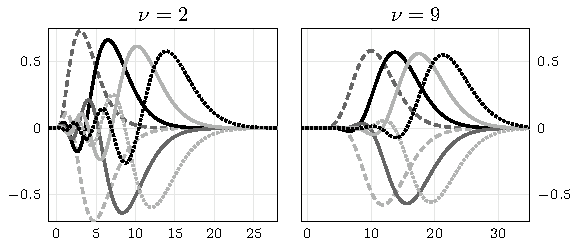
\includegraphics{Figures/fig_matern_non_null_basis.pdf}}\label{fig:matern-non-null-space}
  \end{center}
  \caption{The Mat{\'e}rn--Laguerre functions $\psi_{m, \nu}^+$
  in~\eqref{eq:psi-positive} for $m = 0, \ldots, 6$. Observe that the
  functions vanish on the negative real line.}
\end{figure}

The Mat{\'e}rn expansion~\eqref{eq:matern-expansion} can now be written in
terms of these functions and kernels as
\[ r_{\nu + 1 / 2} (t, u) = \sum_{m = 0}^{\nu} \psi_{m, \nu}^0 (t) \psi_{m,
   \nu}^0 (u) + \rho_{\nu + 1 / 2}^- (t, u) + \rho_{\nu + 1 / 2}^+ (t, u) . \]
It is clear that the functions in $\mathscr{M}_{\nu}^-$ are supported on the
negative real line and the functions in $\mathscr{M}_{\nu}^+$ on the positive
real line. This observation yields the following simplifications:

\begin{align}
  r_{\nu + 1 / 2} (t, u) & = \sum_{m = 0}^{\nu} \psi_{m, \nu}^0 (t) \psi_{m,
  \nu}^0 (u) + \rho_{\nu + 1 / 2}^+ (t, u) &  & \text{if } \quad t \geq 0
  \hspace{0.22em} \text{or } \hspace{0.22em} u \geq 0, 
  \label{eq:matern-simplification-positive}\\
  r_{\nu + 1 / 2} (t, u) & = \sum_{m = 0}^{\nu} \psi_{m, \nu}^0 (t) \psi_{m,
  \nu}^0 (u) + \rho_{\nu + 1 / 2}^- (t, u) &  & \text{if } \quad t \leq 0
  \hspace{0.22em} \text{or } \hspace{0.22em} u \leq 0, \\
  r_{\nu + 1 / 2} (t, u) & = \sum_{m = 0}^{\nu} \psi_{m, \nu}^0 (t) \psi_{m,
  \nu}^0 (u) &  & \text{if } \quad \mathrm{sign} t \neq \mathrm{sign} u. 
  \label{eq:matern-simplification-sign}
\end{align}

We next show that $\mathscr{M}_{\nu}$, $\mathscr{M}_{\nu}^-$, and
$\mathscr{M}_{\nu}^+$ form orthogonal bases with respect to the weight
function
\[ w_{\nu} (t) = 2 / \abs{2 t}^{\nu + 1} . \]
This justifies saying that the expansions we have derived for Mat{\'e}rn
kernels are ``almost'' Mercer.

\begin{proposition}
  [Mat{\'e}rn--Laguerre orthogonality]\label{prop:matern_laguerre_L2}The sets
  $\mathscr{M}_{\nu}$, $\mathscr{M}_{\nu}^+$, and $\mathscr{M}_{\nu}^-$ form
  orthogonal bases in $\mathscr{L}_2 (\mathbb{R}, w_{\nu})$, $\mathscr{L}_2
  (\mathbb{R}_+, w_{\nu})$, and $\mathscr{L}_2 (\mathbb{R}_-, w_{\nu})$,
  respectively. Furthermore,
  \[ \normstar{1}{\psi^+_{m, \nu}}_{\mathscr{L}_2 (\mathbb{R}, w_{\nu})}^2 =
     \normstar{1}{\psi^-_{m, \nu}}_{\mathscr{L}_2 (\mathbb{R}, w_{\nu})}^2 =
     \frac{(\nu !)^2}{(2 \nu) !}  \frac{m!}{(m + \nu + 1) !}  \quad \text{for
     every } \quad m \in \N_0 . \]
\end{proposition}

\begin{proof}
  That $\mathscr{M}_{\nu}^+$ forms an orthogonal basis in $\mathscr{L}_2
  (\mathbb{R}_+, w_{\nu})$ follows from the fact that the functions
  \begin{equation}
    t^{\nu / 2 + 1 / 2} \mathrm{L}_m^{(\nu + 1)} (t) e^{- t / 2}  \quad
    \text{for } \quad m \in \N_0
  \end{equation}
  form an orthonormal basis in $\mathscr{L}_2 (\mathbb{R}_+)$
  {\citep{Szego1939}}. Furthermore, the norms of the functions in
  $\mathscr{M}_{\nu}^+$ are readily computed from the norms of the
  corresponding Laguerre polynomials:
  \[ \begin{eqsplit}
       \normstar{1}{\psi^+_{m, \nu}}_{\mathscr{L}_2 (\mathbb{R}, w_{\nu})}^2 &
       = \frac{(\nu !)^2}{(2 \nu) !} \left( \frac{m!}{(m + \nu + 1) !}
       \right)^2  \int_0^{\infty} [\mathrm{L}_m^{(\nu + 1)} (t)]^2 t^{\nu + 1}
       e^{- t} \dif t\\
       & = \frac{(\nu !)^2}{(2 \nu) !}  \frac{m!}{(m + \nu + 1) !} .
     \end{eqsplit} \]
  The statement pertaining to $\mathscr{M}_{\nu}^-$ follows from the symmetry
  \eqref{eq:negative_matern_laguerre} and the statement pertaining to
  $\mathscr{M}_{\nu}$ from the fact that $\mathscr{L}_2 (\mathbb{R}) =
  \mathscr{L}_2 (\mathbb{R}_-) \oplus \mathscr{L}_2 (\mathbb{R}_+)$.
\end{proof}

{\rev{Because they do not decay to zero sufficiently fast at the origin, the
functions in $\mathscr{M}_{\nu}^0$ are not members of $\mathscr{L}_2
(\mathbb{R}, w_{\nu})$. This will become evident in
Section~\ref{sec:null-space}. }}

\subsection{Truncation error}

\begin{figure}[h]
  \begin{center}
    \resizebox{1\columnwidth}{!}{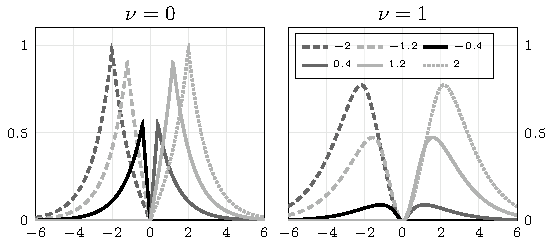
\includegraphics{Figures/fig_matern_rho_kernel.pdf}}\label{fig:matern-rho-kernel}
  \end{center}
  \caption{Translates $\rho_{\nu + 1 / 2} (\cdummy, u)$ of the kernel
  in~\eqref{eq:rho-kernel} for $u \in \{- 2, - 1.2, - 0.4, 0.4, 1.2, 2\}$.
  Observe that each translate is supported on the axis that $u$ lies on.}
\end{figure}

Define the kernel
\begin{equation}
  \label{eq:rho-kernel} \rho_{\nu + 1 / 2} (t, u) = \rho_{\nu + 1 / 2}^- (t,
  u) + \rho_{\nu + 1 / 2}^+ (t, u)
\end{equation}
in terms of the kernels in~\eqref{eq:rho-kernels}. A few translates of this
kernel are displayed in  Figure~\ref{fig:matern-rho-kernel}. The full
Mat{\'e}rn kernel is therefore
\[ r_{\nu + 1 / 2} (t, u) = \sum_{m = 0}^{\nu} \psi_{m, \nu}^0 (t) \psi_{m,
   \nu}^0 (u) + \rho_{\nu + 1 / 2} (t, u) . \]
From  Proposition~\ref{prop:matern_laguerre_L2} we see that the kernel
$\rho_{\nu + 1 / 2}$ is an element of $\mathscr{L}_2 (\mathbb{R} \times
\mathbb{R}, w_{\nu} \otimes w_{\nu})$ and that its squared norm is given by
\[ \begin{eqsplit}
     \int_{- \infty}^{\infty} \int_{- \infty}^{\infty} \rho_{\nu + 1 / 2}^2 &
     (t, u) w_{\nu} (t) w_{\nu} (u) \dif t \dif u\\
     & = \sum_{m = 0}^{\infty} \left( \normstar{1}{\psi^-_{m,
     \nu}}_{\mathscr{L}_2 (\mathbb{R}, w_{\nu})}^4 + \normstar{1}{\psi^+_{m,
     \nu}}_{\mathscr{L}_2 (\mathbb{R}, w_{\nu})}^4 \hspace{-0.17em} \right) .
   \end{eqsplit} \]
This implies that $\rho_{\nu + 1 / 2}$ defines a Hilbert--Schmidt operator on
$\mathscr{L}_2 (\mathbb{R}, w_{\nu})$ via~\eqref{eq:mercer-integral-operator}
and that the above norm is precisely the squared Hilbert--Schmidt norm of this
operator~{\citep{Kuo1975}}. Next the approximation errors for appropriately
truncated approximations of the Mat{\'e}rn kernel are examined in terms of the
Hilbert--Schmidt norm. Let $n \geq 1$ and define the truncated kernels

\begin{align}
  \rho_{\nu + 1 / 2, n} (t, u) & = \sum_{m = 0}^{n - 1} \psi_{m, \nu}^- (t)
  \psi_{m, \nu}^- (u) + \sum_{m = 0}^{n - 1} \psi_{m, \nu}^+ (t) \psi_{m,
  \nu}^+ (u), \\
  r_{\nu + 1 / 2, n} (t, u) & = \sum_{m = 0}^{\nu} \psi_{m, \nu}^0 (t)
  \psi_{m, \nu}^0 (u) + \rho_{\nu + 1 / 2, n} (t, u) . 
  \label{eq:matern-truncation}
\end{align}

Observe that $r_{\nu + 1 / 2, n}$ is a finite expansion of $\nu + 1 + 2 n$
terms. Some truncations of Mat{\'e}rn kernels are displayed in 
Figure~\ref{fig:matern-truncations}.

\begin{figure}[h]
  \begin{center}
    \resizebox{1\columnwidth}{!}{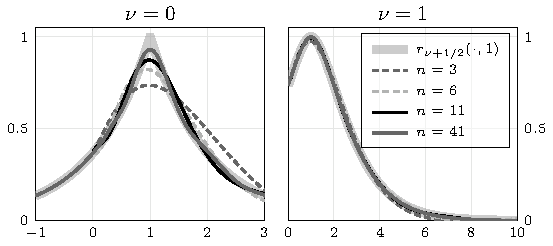
\includegraphics{Figures/fig_matern_truncations.pdf}}\label{fig:matern-truncations}
  \end{center}
  \caption{The truncation in~\eqref{eq:matern-truncation} for two Mat{\'e}rn
  kernels. Because the second kernel argument has been fixed to a positive
  value, the truncations are exact on the negative real line
  by~\eqref{eq:matern-simplification-sign}.}
\end{figure}

\begin{proposition}
  [Mat{\'e}rn truncation]\label{prop:matern-truncation-error}For every $n \in
  \N$ it holds that
  \[ \left( \int_{- \infty}^{\infty} \int_{- \infty}^{\infty} (r_{\nu + 1 / 2}
     (t, u) - r_{\nu + 1 / 2, n} (t, u))^2 w_{\nu} (t) w_{\nu} (u) \dif t \dif
     u \right)^{1 / 2} \leq \frac{c_{\nu}}{n^{\nu + 1 / 2}}, \]
  where
  \[ c_{\nu} = \frac{(\nu !)^2}{(2 \nu) !}  \sqrt{\frac{2 (2 \nu + 2)}{2 \nu +
     1}} \sim \frac{1}{2^{2 \nu}}  \sqrt{\frac{2 \pi (2 \nu + 2) \nu}{2 \nu +
     1}}  \quad \text{as } \quad \nu \to \infty . \]
\end{proposition}

\begin{proof}
  Firstly, the truncation error is
  \[ \begin{eqsplit}
       r_{\nu + 1 / 2} (t, u) - r_{\nu + 1 / 2, n} (t, u) & = \rho_{\nu + 1 /
       2} (t, u) - \rho_{\nu + 1 / 2, n} (t, u)\\
       & = \sum_{m = n}^{\infty} [\psi^-_{m, \nu} (t) \psi^-_{m, \nu} (u) +
       \psi^+_{m, \nu} (t) \psi^+_{m, \nu} (u)] .
     \end{eqsplit} \]
  Using  Proposition~\ref{prop:matern_laguerre_L2}, the squared norm of the
  truncation error is straight-forwardly computed as
  \[ \begin{eqsplit}
       \int_{- \infty}^{\infty} \int_{- \infty}^{\infty} (r_{\nu + 1 / 2} &
       (t, u) - r_{\nu + 1 / 2, n} (t, u))^2 w_{\nu} (t) w_{\nu} (u) \dif t
       \dif u\\
       & = \sum_{m = n}^{\infty} \left( \normstar{1}{\psi^-_{m,
       \nu}}_{\mathscr{L}_2 (\mathbb{R}, w_{\nu})}^4 + \normstar{1}{\psi^+_{m,
       \nu}}_{\mathscr{L}_2 (\mathbb{R}, w_{\nu})}^4 \right)\\
       & = 2 \left( \frac{(\nu !)^2}{(2 \nu) !} \right)^2  \sum_{m =
       n}^{\infty} \left( \frac{m!}{(m + \nu + 1) !} \right)^2\\
       & \leq 2 \left( \frac{(\nu !)^2}{(2 \nu) !} \right)^2  \sum_{m =
       n}^{\infty} \frac{1}{m^{2 \nu + 2}} .
     \end{eqsplit} \]
  The sum may be estimated with an integral as
  \[ \begin{eqsplit}
       \sum_{m = n}^{\infty} \frac{1}{m^{2 \nu + 2}} & \leq \frac{1}{n^{2 \nu
       + 2}} + \int_n^{\infty} \frac{1}{t^{2 \nu + 2}} \dif t = \frac{1}{n^{2
       \nu + 2}} + \frac{1}{2 \nu + 1}  \hspace{0.17em} \frac{1}{n^{2 \nu +
       1}} \leq \frac{2 \nu + 2}{2 \nu + 1}  \hspace{0.17em} \frac{1}{n^{2 \nu
       + 1}},
     \end{eqsplit} \]
  where $n \geq 1$ was used in the last inequality. This yields the desired
  upper bound. The asymptotic equivalence for $c_{\nu}$ as $\nu \to \infty$
  follows from Stirling's formula.
\end{proof}

\subsection{The null-space $\mathscr{M}_{\nu}^0$}\label{sec:null-space}

\begin{figure}[h]
  \begin{center}
    \resizebox{1\columnwidth}{!}{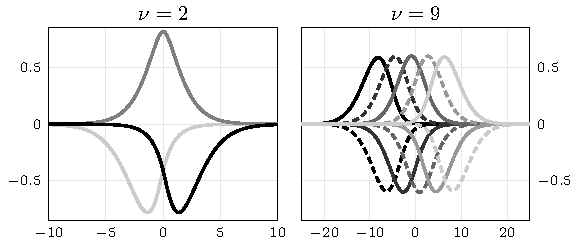
\includegraphics{Figures/fig_matern_null_basis.pdf}}\label{fig:matern-null-space}
  \end{center}
  \caption{The null-space Mat{\'e}rn--Laguerre functions $\psi_{m, \nu}^0$
  in~\eqref{eq:psi-null} for $\nu = 2$ and $\nu = 9$.}
\end{figure}

In view of  Proposition~\ref{prop:matern_laguerre_L2}, $\mathscr{M}_{\nu}^0$
is left as the odd set out. From~\eqref{eq:h-hat-matern} and
\eqref{eq:matern_laguerre_functions} we compute that
\[ \label{eq:nullspace_functions} \hat{\psi}^0_{m, \nu} (\omega) = (- 1)^{\nu
   + 1}  \hat{h}_{\nu + 1 / 2}^{\ast} (\omega)  \hat{\varphi}_m (\omega) . \]
Furthermore, the functions
\[ (i \omega + 1)^{\nu + 1}  \hat{\psi}^0_{m, \nu} (\omega), \]
when viewed as functions of $i \omega$, have no poles in the left half-plane.
Therefore $\smash{[} b] \mathscr{M}_{\nu}^0$ are annihilated on the positive
real line by the differential operator $\smash{[} b] (\mathrm{D} + 1)^{\nu +
1}$. That is,
\[ (\mathrm{D} + 1)^{\nu + 1} \psi_{m, \nu}^0 (t) = 0 \quad \text{for every }
   \quad t > 0. \]
For this reason we refer to these functions as the null-space functions. The
null space functions have a symmetry property similar to that of the functions
$\mathscr{M}_{\nu}$ given by~\eqref{eq:psi-positive}
and~\eqref{eq:psi-negative}.

\begin{proposition}
  [Null-space symmetry] The null-space functions satisfy
  \[ \psi^0_{\nu - m, \nu} (t) = (- 1)^{\nu} \psi^0_{m, \nu}  (- t)  \quad
     \text{and } \quad \hat{\psi}^0_{\nu - m, \nu} (\omega) = (- 1)^{\nu} 
     \hat{\psi}^{0 \ast}_{m, \nu} (\omega) . \]
  for $m = 0, 1, \ldots, \nu$.
\end{proposition}

\begin{proof}
  Starting from \eqref{eq:matern_laguerre_binomial_expression}, using the
  conjugate symmetry of Laguerre functions, and then changing the order of
  summation gives
  \[ \begin{eqsplit}
       \hat{\psi}^0_{m, \nu} (\omega) & = \frac{1}{\sqrt{\smash{[} b] 2}} 
       \frac{\nu !}{\sqrt{\smash{[} b] (2 \nu) !}}  \sum_{k = 0}^{\nu + 1}
       \binom{\nu + 1}{k} (- 1)^k  \hat{\varphi}_{- \nu - 1 + m + k}
       (\omega)\\
       & = \frac{1}{\sqrt{\smash{[} b] 2}}  \frac{\nu !}{\sqrt{\smash{[} b]
       (2 \nu) !}}  \sum_{k = 0}^{\nu + 1} \binom{\nu + 1}{k} (- 1)^k 
       \hat{\varphi}_{- (\nu - m - k) - 1} (\omega)\\
       & = - \frac{1}{\sqrt{\smash{[} b] 2}}  \frac{\nu !}{\sqrt{\smash{[} b]
       (2 \nu) !}}  \sum_{k = 0}^{\nu + 1} \binom{\nu + 1}{k} (- 1)^k 
       \hat{\varphi}_{\nu - m - k}^{\ast} (\omega)\\
       & = - \frac{1}{\sqrt{\smash{[} b] 2}}  \frac{\nu !}{\sqrt{\smash{[} b]
       (2 \nu) !}}  \sum_{k = 0}^{\nu + 1} \binom{\nu + 1}{\nu + 1 - k} (-
       1)^{\nu + 1 - k}  \hat{\varphi}_{\nu - m - (\nu + 1 - k)}^{\ast}
       (\omega)\\
       & = (- 1)^{\nu} \frac{1}{\sqrt{\smash{[} b] 2}}  \frac{\nu
       !}{\sqrt{\smash{[} b] (2 \nu) !}}  \sum_{k = 0}^{\nu + 1} \binom{\nu +
       1}{k} (- 1)^k  \hat{\varphi}_{- \nu - 1 + \nu - m + k}^{\ast}
       (\omega)\\
       & = (- 1)^{\nu}  \hat{\psi}^{0 \ast}_{\nu - m, \nu} (\omega),
     \end{eqsplit} \]
  which is the Fourier domain symmetry. The time domain symmetry is then
  obtained from Fourier inversion.
\end{proof}

\begin{example}
  [Null-space functions]\label{example:null-space}The set $\mathscr{M}_0^0$
  (i.e., $\nu = 0$) consists of the function
  \[ \psi^{0, (0)}_0 (t) = - e^{- \absstar{0}{t}} . \]
  The set $\mathscr{M}_1^0$ (i.e., $\nu = 1$) consists of the functions
  \[ \psi^0_{0, 1} (t) = \frac{1}{\sqrt{\smash{[} b] 2}}  (2 te^t 
     \textbf{1}_{(- \infty, 0)} (t) + e^{- \absstar{0}{t}})  \quad \text{and }
     \quad \psi^0_{1, 1} (t) = - \frac{1}{\sqrt{\smash{[} b] 2}}  (2 te^{- t} 
     \textbf{1}_{[0, \infty)} (t) + e^{- \absstar{0}{t}}) . \]
  The set $\mathscr{M}_2^0$ (i.e., $\nu = 2$) consists of the functions
  
  \begin{align*}
    \psi^0_{0, 2} (t) & = \frac{2}{\sqrt{\smash{[} b] 4!}}  \left( 2 (- t^2 +
    t) e^t  \textbf{1}_{(- \infty, 0)} (t) - e^{- \absstar{0}{t}} \right),\\
    \psi^0_{1, 2} (t) & = \frac{4}{\sqrt{\smash{[} b] 4!}}  (\absstar{0}{t} +
    1) e^{- \absstar{0}{t}},\\
    \psi^0_{2, 2} (t) & = \frac{2}{\sqrt{\smash{[} b] 4!}}  \left( - 2 (t^2 +
    t) e^{- t}  \textbf{1}_{[0, \infty)} (t) - e^{- \absstar{0}{t}} \right) .
  \end{align*}
\end{example}

Some null space functions are depicted in  Figure~\ref{fig:matern-null-space}.
Unlike the basis functions $\mathscr{M}_{\nu}^+$ depicted in 
Figure~\ref{fig:matern-non-null-space}, the null space functions are supported
on the entire real line. For $d = \absstar{0}{t - u}$, a Mat{\'e}rn kernel can
be written as
\[ r_{\nu + 1 / 2} (t, u) = r_{\nu + 1 / 2} (0, d) = \sum_{m = 0}^{\nu}
   \psi_{m, \nu}^0 (0) \psi_{m, \nu}^0 (d), \]
where we have used~\eqref{eq:matern-simplification-positive} and the fact that
the kernel $\rho_{\nu + 1 / 2}^+ (t, u)$ vanishes if $t = 0$ or $u = 0$. Upon
substitution of the expressions in  Example~\ref{example:null-space} we obtain
the well-known explicit forms of Mat{\'e}rn kernels in terms of $d$, such as
\[ r_{3 / 2} (t, u) = (1 + d) e^{- d}  \quad \text{and } \quad r_{5 / 2} (t,
   u) = \left( 1 + d + \frac{d^2}{3} \right) e^{- d} . \]
\section{Expansions of the Cauchy kernel}\label{sec:cauchy}

The Cauchy kernel and its Fourier transform are
\begin{equation}
  \label{eq:cauchy-kernel} r (t, u) = \frac{1}{1 + (t - u)^2}  \quad \text{and
  } \quad \hat{\Phi} (\omega) = \pi e^{- \absstar{0}{\omega}} .
\end{equation}
The Cauchy kernel is thus a Fourier dual to the Mat{\'e}rn kernel of
smoothness index $\alpha = 1 / 2$ (i.e., $\nu = 0$). In what follows this will
inform the construction of an RKHS basis. A square-root of $\hat{\Phi}
(\omega)$ is then given by
\begin{equation}
  \label{eq:h-cauchy} \hat{h} (\omega) = \hat{\Phi} (\omega)^{1 / 2} =
  \sqrt{\pi}  \hspace{0.17em} e^{- \absstar{0}{\omega} / 2} .
\end{equation}
\subsection{Expansion in complex-valued Cauchy--Laguerre
functions}\label{sec:cauchy-complex}

In view of the Fourier dualism with the Mat{\'e}rn-$\frac{1}{2}$ kernel and
the fact that the Fourier transform is an isometry from $\mathscr{L}_2 (\R)$
to $\mathscr{L}_2 (\R, 1 / 2 \pi)$, a straight-forward way to construct a
suitable basis of $\mathscr{L}_2 (\R)$ for Theorem~\ref{thm:main-theorem} is
to modify the Laguerre functions from  Section~\ref{sec:laguerre-functions}
and consider the functions $\sqrt{\pi} \varphi_m  (\omega / 2)$. The Fourier
transforms of these functions are an orthonormal basis of $\mathscr{L}_2
(\R)$, so that Theorem~\ref{thm:main-theorem} and~\eqref{eq:h-cauchy} yield
the RKHS basis functions
\[ \hat{\psi}_m (\omega) = \sqrt{\pi}  \hspace{0.17em} e^{-
   \absstar{0}{\omega} / 2}  \sqrt{\pi}  \hspace{0.17em} \varphi_m  (\omega /
   2) \]
in the Fourier domain. Since their inverse Fourier transforms are
complex-valued, we call these functions the {\tmem{complex-valued
Cauchy--Laguerre functions}}. For $m \in \N_0$, Fourier inversion gives
\[ \begin{eqsplit}
     \psi_m (t) = \frac{1}{2}  \int_{- \infty}^{\infty} e^{-
     \absstar{0}{\omega} / 2} \varphi_m  (\omega / 2) e^{i \omega t} \dif
     \omega & = \int_{- \infty}^{\infty} e^{- \absstar{0}{\omega}} \varphi_m
     (\omega) e^{i \omega 2 t} \dif \omega\\
     & = \int_0^{\infty} e^{- \absstar{0}{\omega}} \varphi_m (\omega) e^{i
     \omega 2 t} \dif \omega\\
     & = \int_0^{\infty} e^{- \absstar{0}{\omega}} \varphi_m (\omega) e^{- i
     \omega (- 2 t - i)} \dif \omega\\
     & = \hat{\varphi}_m  (- 2 t - i)\\
     & = - \frac{1}{\sqrt{2}}  \frac{(it)^m}{(it - 1)^{m + 1}} .
   \end{eqsplit} \]
Similarly, for negative indices we get
\[ \begin{eqsplit}
     \psi_{- m} (t) = \frac{1}{2}  \int_{- \infty}^{\infty} e^{-
     \absstar{0}{\omega} / 2} \varphi_{- m}  (\omega / 2) e^{i \omega t} \dif
     \omega & = \int_{- \infty}^{\infty} e^{- \absstar{0}{\omega}} \varphi_{-
     m} (\omega) e^{i \omega 2 t} \dif \omega\\
     & = - \int_{- \infty}^0 e^{- \absstar{0}{\omega}} \varphi_{m - 1}  (-
     \omega) e^{i \omega 2 t} \dif \omega\\
     & = - \int_0^{\infty} e^{- \absstar{0}{\omega}} \varphi_{m - 1} (\omega)
     e^{- i \omega 2 t} \dif \omega\\
     & = - \int_0^{\infty} \varphi_{m - 1} (\omega) e^{- i \omega (2 t - i)}
     \dif \omega\\
     & = - \hat{\varphi}_{m - 1}  (2 t - i)\\
     & = - \frac{1}{\sqrt{2}}  \frac{(it)^{m - 1}}{(it + 1)^m} .
   \end{eqsplit} \]
To summarise, the complex valued Cauchy--Laguerre functions are

{\subequations{\label{eq:cauch-laguerre-funcs}

\begin{align}
  \psi_m (t) & = - \frac{1}{\sqrt{2}}  \frac{(it)^m}{(it - 1)^{m + 1}}  \quad
  \text{for } \quad m \in \mathbb{N}_0, \\
  \psi_{- m - 1} (t) & = - \frac{1}{\sqrt{2}}  \frac{(it)^m}{(it + 1)^{m + 1}}
  \quad \text{for } \quad m \in \mathbb{N}_0 . 
\end{align}}}

They have the conjugate symmetry property
\[ \psi_m^{\ast} (t) = - \psi_{- m - 1} (t) = \psi_m  (- t)  \quad \text{for }
   \quad m \in \Z . \]
An expansion of the Cauchy kernel~\eqref{eq:cauchy-kernel} in terms of
complex-valued Cauchy--Laguerre functions is thus given by
\[ r (t, u) = \sum_{m = - \infty}^{\infty} \psi_m^{\ast} (t) \psi_m (u) . \]
This expansion is remarkably easy to verify by independent means since
geometric summation and conjugate symmetry yield
\[ \sum_{m = 0}^{\infty} \psi_m^{\ast} (t) \psi_m (u) = \frac{1}{2} 
   \frac{1}{(it - 1)  (- iu - 1) - tu} \]
and
\[ \sum_{m = - \infty}^{- 1} \psi_m^{\ast} (t) \psi_m (u) = \left( \sum_{m =
   0}^{\infty} \psi_m^{\ast} (t) \psi_m (u) \right)^{\ast} . \]
Hence
\[ \begin{eqsplit}
     \sum_{m = - \infty}^{\infty} \psi_m^{\ast} (t) \psi_m (u) = \frac{1}{2} 
     \frac{1}{1 - i (t - u)} + \frac{1}{2}  \frac{1}{1 + i (t - u)} =
     \frac{1}{1 + (t - u)^2},
   \end{eqsplit} \]
which indeed is the Cauchy kernel. An appropriate $\mathscr{L}_2 (\R, w)$
space in which the complex-valued Cauchy--Laguerre functions form a complete
orthogonal set remains elusive to us. However, just as with the
Mat{\'e}rn--Laguerre expansions in  Section~\ref{sec:matern}, the present
expansion is very good at origin since all but two terms vanish:
\[ r (t, 0) = \sum_{m = - \infty}^{\infty} \psi_m^{\ast} (t) \psi_m (0) = -
   (\psi_{- 1} (t) + \psi_0 (t)) . \]
\subsection{Expansion in {\rev{real-valued Cauchy--Laguerre
functions}}}\label{sec:cauchy-real}

\begin{figure}[h]
  \begin{center}
    \resizebox{1\columnwidth}{!}{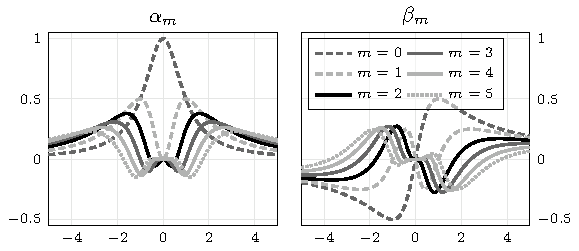
\includegraphics{Figures/fig_cauchy_basis.pdf}}\label{fig:cauchy-basis}
  \end{center}
  \caption{The {\rev{real-valued Cauchy--Laguerre functions}} $\alpha_m$ and
  $\beta_m$ in~\eqref{eq:trig-cauchy-laguerre}.}
\end{figure}

It would be desirable to obtain a real-valued basis for the Cauchy RKHS. This
can be done by scaling the real and imaginary parts of $\hat{\psi}_m$ in a
similar manner as was done for the Laguerre functions
in~{\cite{Christov1982}}. This gives the RKHS basis functions
\begin{equation}
  \label{eq:trig-cauchy-laguerre} \alpha_m (t) = \frac{1}{\sqrt{2}}  (\psi_m
  (t) + \psi_m^{\ast} (t))  \quad \text{and } \quad \beta_m (t) = \frac{1}{i
  \sqrt{2}}  (\psi_m (t) - \psi_m^{\ast} (t))
\end{equation}
for $m \in \N_0$, where $\psi_m$ are the complex-valued Cauchy--Laguerre
functions in~\eqref{eq:cauch-laguerre-funcs}. We call the functions $\alpha_m$
and $\beta_m$ the {\tmem{{\rev{real-valued Cauchy--Laguerre functions}}}}. The
binomial theorem yields the explicit expressions

\begin{align*}
  \alpha_m (t) & = \frac{1}{2}  \frac{(- 1)^m  (it)^m}{(t^2 + 1)^{m + 1}} 
  \sum_{k = 0}^{m + 1} \binom{m + 1}{k} (it)^k  (1 - (- 1)^{m + 1 - k}),\\
  \beta_m (t) & = \frac{1}{i 2}  \frac{(- 1)^m  (it)^m}{(t^2 + 1)^{m + 1}} 
  \sum_{k = 0}^{m + 1} \binom{m + 1}{k} (it)^k  (1 + (- 1)^{m + 1 - k}),
\end{align*}

which can be transformed into expressions of only real parameters by
considering even and odd $m$ separately. This yields

{\subequations{\label{eq:real_cauchy_laguerre_explicit}

\begin{align}
  \alpha_{2 m} (t) & = \frac{(- 1)^m t^{2 m}}{(t^2 + 1)^{2 m + 1}}  \sum_{k =
  0}^m \binom{2 m + 1}{2 k} (- 1)^k t^{2 k}, \\
  \alpha_{2 m + 1} (t) & = \frac{(- 1)^m t^{2 m + 1}}{(t^2 + 1)^{2 m + 2}} 
  \sum_{k = 0}^m \binom{2 m + 2}{2 k + 1} (- 1)^k t^{2 k + 1}, \\
  \beta_{2 m} (t) & = \frac{(- 1)^m t^{2 m}}{(t^2 + 1)^{2 m + 1}}  \sum_{k =
  0}^m \binom{2 m + 1}{2 k + 1} (- 1)^k t^{2 k + 1}, \\
  \beta_{2 m + 1} (t) & = \frac{(- 1)^{m + 1} t^{2 m + 1}}{(t^2 + 1)^{2 m +
  2}}  \sum_{k = 0}^{m + 1} \binom{2 m + 2}{2 k} (- 1)^k t^{2 k} . 
\end{align}}}

An expansion of the Cauchy kernel~\eqref{eq:cauchy-kernel} in terms of real
functions is thus given by
\begin{equation}
  \label{eq:cauchy-expansion-trig} r (t, u) = \sum_{m = 0}^{\infty} \alpha_m
  (t) \alpha_m (u) + \sum_{m = 0}^{\infty} \beta_m (t) \beta_m (u) .
\end{equation}
At the origin, this reduces to the finite term expansion
\[ r (t, 0) = \alpha_0 (t) \alpha_0 (0) . \]
The basis functions $\alpha_m$ and $\beta_m$ and truncations of the
expansion~\eqref{eq:cauchy-expansion-trig} are displayed in 
Figures~\ref{fig:cauchy-basis} and~\ref{fig:cauchy-truncation}.

\begin{figure}[h]
  \begin{center}
    \resizebox{1\columnwidth}{!}{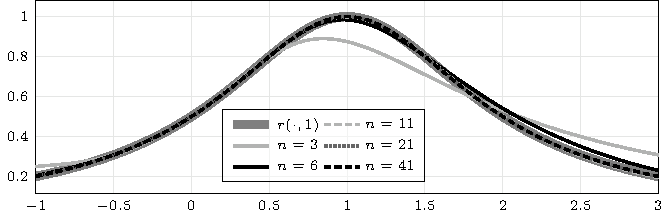
\includegraphics{Figures/fig_cauchy_truncation.pdf}}\label{fig:cauchy-truncation}
  \end{center}
  \caption{Truncations $\sum_{m = 0}^{n - 1} \alpha_m (t) \alpha_m (u) +
  \sum_{m = 0}^{n - 1} \beta_m (t) \beta_m (u)$ of the Cauchy expansion
  in~\eqref{eq:cauchy-expansion-trig}.}
\end{figure}

\section{Expansion of the Gaussian kernel}\label{sec:gaussian}

The Gaussian kernel and its Fourier transform are
\begin{equation}
  \label{eq:gaussian-kernel} r (t, u) = \exp \left( \hspace{-0.17em} -
  \frac{1}{2} (t - u)^2 \right)  \quad \text{and } \quad \hat{\Phi} (\omega) =
  \sqrt{2 \pi}  \hspace{0.17em} e^{- \omega^2 / 2} .
\end{equation}
A square-root is
\[ \hat{h} (\omega) = \hat{\Phi} (\omega)^{1 / 2} = (2 \pi)^{1 / 4} e^{-
   \omega^2 / 4}, \]
so that taking the inverse Fourier transform gives the function $h$ in 
Theorem~\ref{thm:main-theorem} as
\begin{equation}
  \label{eq:h-gaussian} h (t) = 2^{1 / 4} \pi^{- 1 / 4} e^{- t^2} .
\end{equation}
\subsection{Expansion for the Gaussian kernel}\label{sec:gaussian-expansion}

As an orthonormal basis of $\mathscr{L}_2 (\R)$ we use the {\tmem{Hermite
functions}} (for them being an orthonormal basis,
see~{\cite[Theorem~5.7.1]{Szego1939}})
\begin{equation}
  \label{eq:hermite-function} \varphi_m (t) = \sqrt{\frac{1}{2^m m!
  \sqrt{\pi}}}  \hspace{0.17em} e^{- t^2 / 2} \mathrm{H}_m (t)  \quad
  \text{for } \quad m \in \N_0 .
\end{equation}
Here $\mathrm{H}_m$ is the $m$th physicist's Hermite polynomial given by
\begin{equation}
  \label{eq:hermite-polynomial} \mathrm{H}_m (t) = m! \sum_{k = 0}^{\lfloor m
  / 2 \rfloor} \frac{(- 1)^k}{k! (m - 2 k) !}  (2 t)^{m - 2 k} .
\end{equation}
By  Theorem~\ref{thm:main-theorem}, the functions
\[ \psi_m (t) = \int_{- \infty}^{\infty} h (t - \tau) \varphi_m (\tau) \dif
   \tau = \left( \frac{\sqrt{2}}{\pi} \right)^{1 / 2} \sqrt{\frac{1}{2^m m!}} 
   \int_{- \infty}^{\infty} e^{- (t - \tau)^2} e^{- \tau^2 / 2} \mathrm{H}_m
   (\tau) \dif \tau \]
form an orthonormal basis of the RKHS of the Gaussian
kernel~\eqref{eq:gaussian-kernel}. Equation~(17) in Section~16.5
of~{\cite{Erdelyi1954}} states that
\[ \int_{- \infty}^{\infty} e^{- (s - \tau)^2} \mathrm{H}_m (a \tau) \dif \tau
   = \sqrt{\pi}  (1 - a^2)^{m / 2} \mathrm{H}_m \left( \frac{as}{\sqrt{1 -
   a^2}} \right) \]
for any reals $s$ and $a$. Completing the square, doing a change of variables,
and using this equation yields
\[ \begin{eqsplit}
     \int_{- \infty}^{\infty} e^{- (t - \tau)^2} e^{- \tau^2 / 2} \mathrm{H}_m
     (\tau) \dif \tau & = \sqrt{\frac{2}{3}} e^{- t^2 / 3}  \int_{-
     \infty}^{\infty} e^{- (\sqrt{\smash{[} b] 2 / 3}  \hspace{0.17em} t -
     \tau)^2} \mathrm{H}_m \left( \sqrt{\smash{[} b] 2 / 3}  \hspace{0.17em}
     \tau \right) \dif \tau\\
     & = \sqrt{\frac{2 \pi}{3}} 3^{- m / 2} e^{- t^2 / 3} \mathrm{H}_m \left(
     \frac{2 t}{\sqrt{3}} \right) .
   \end{eqsplit} \]
We thus obtain the basis functions
\begin{equation}
  \label{eq:gaussian-basis} \psi_m (t) = \left( \frac{2 \sqrt{2}}{3}
  \right)^{1 / 2} \sqrt{\frac{1}{6^m m!}} e^{- t^2 / 3} \mathrm{H}_m \left(
  \frac{2 t}{\sqrt{3}} \right)  \quad \text{for } \quad m \in \N_0
\end{equation}
and the resulting expansion
\begin{equation}
  \label{eq:gaussian-expansion} r (t, u) = \sum_{m = 0}^{\infty} \psi_m (t)
  \psi_m (u)
\end{equation}
of the Gaussian kernel in~\eqref{eq:gaussian-kernel}. 
Figure~\ref{fig:gaussian-basis} displays some of the basis functions.

\begin{figure}[h]
  \begin{center}
    \resizebox{1\columnwidth}{!}{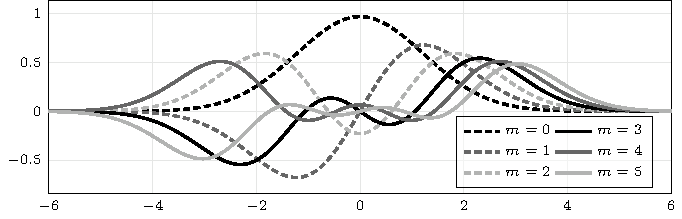
\includegraphics{Figures/fig_gaussian_basis.pdf}}\label{fig:gaussian-basis}
  \end{center}
  \caption{The first six basis functions $\psi_m$ in~\eqref{eq:gaussian-basis}
  of the Gaussian kernel~\eqref{eq:gaussian-kernel}.}
\end{figure}

Note that the basis functions can be written in terms of the Hermite
functions~\eqref{eq:hermite-function} by using the multiplication theorem
\[ \mathrm{H}_m (bt) = \sum_{k = 0}^{\lfloor m / 2 \rfloor} b^{m - 2 k}  (b^2
   - 1)^k \binom{m}{2 k} \frac{(2 k) !}{k!} \mathrm{H}_{m - 2 k} (t) \]
for Hermite polynomials. Setting $b = \sqrt{2}$ gives
\[ \mathrm{H}_m \left( \frac{2 t}{\sqrt{3}} \right) = 2^{m / 2}  \sum_{k =
   0}^{\lfloor m / 2 \rfloor} 2^{- k} \binom{m}{2 k} \frac{(2 k) !}{k!}
   \mathrm{H}_{m - 2 k} \left( \frac{\sqrt{2}  \hspace{0.17em} t}{\sqrt{3}}
   \right), \]
so that
\[ \psi_m (t) = \left( \frac{2 \sqrt{\pi}}{\sqrt{3}} \right)^{1 / 2}
   \sqrt{\frac{2^m m!}{3^m}}  \sum_{k = 0}^{\lfloor m / 2 \rfloor}
   \frac{1}{4^k k! \sqrt{(m - 2 k) !}}  \hspace{0.17em} \varphi_{m - 2 k}
   \left( \frac{\sqrt{2}  \hspace{0.17em} t}{\sqrt{3}} \right) . \]
It would be interesting to be able to connect $\psi_m$ to the associated
Hermite polynomials~{\cite{AskeyWimp1984}} like the Mat{\'e}rn--Laguerre
functions are connected to associated Laguerre functions in 
Section~\ref{sec:matern-classification}.

\begin{remark}
  Observe that (both here and elsewhere) we have used a basis of
  $\mathscr{L}_2 (\R)$ that is ``compatible'' with the kernel, having the same
  scaling in the exponential. That is, the Hermite functions
  in~\eqref{eq:hermite-function} have the exponential term $e^{- t^2 / 2}$ and
  the kernel is $e^{- (t - u)^2 / 2}$. For any $\kappa \in (0, \sqrt{2})$, the
  scaled Hermite functions
  \[ \varphi_{m, \kappa} (t) = \sqrt{\frac{\kappa}{2^m m! \sqrt{\pi}}} 
     \hspace{0.17em} e^{- \kappa^2 t^2 / 2} \mathrm{H}_m (\kappa t) \]
  would yield the RKHS basis functions
  \[ \psi_{m, \kappa} (t) = \left( \frac{\sqrt{2} \kappa}{a^2} \right)^{1 / 2}
     \sqrt{\frac{1}{2^m m!}}  \left( 1 - \frac{\kappa^2}{a^2} \right)^{m / 2}
     e^{- (1 - 1 / a^2) t^2} \mathrm{H}_m \left( \frac{\kappa t}{a^2 
     \sqrt{\smash{[} b] 1 - \kappa^2 / a^2}} \right), \]
  where $a^2 = 1 + \kappa^2 / 2$.
\end{remark}

\subsection{Mercer basis and Mehler's formula}

The expansion~\eqref{eq:gaussian-expansion} that we derived for the Gaussian
kernel by the use of the basis functions in~\eqref{eq:gaussian-basis} can also
be derived by setting
\[ \rho = \frac{1}{3}, \quad x = \frac{2 t}{\sqrt{3}}, \quad \text{and } \quad
   y = \frac{2 u}{\sqrt{3}} \]
in Mehler's formula
\[ \sum_{m = 0}^{\infty} \frac{(\rho / 2)^m}{m!} \mathrm{H}_m (x) \mathrm{H}_m
   (y) e^{- (x^2 + y^2) / 2} = \sqrt{\frac{1}{1 - \rho^2}} \exp \left( \frac{4
   xy \rho - (1 + \rho^2) (x^2 + y^2)}{2 (1 - \rho^2)} \right) \]
and subsequently multiplying both sides by $e^{- (t^2 + u^2) / 3}$. This
suggests that the expansion derived in the preceding section is a special case
of the relatively well known Mercer expansion of the Gaussian kernel,
{\rev{which can also be derived}} from Mehler's
formula~{\cite[Section~12.2.1]{FasshauerMcCourt2015}}. Let $\alpha > 0$ and
define the constants
\[ \beta = \left( 1 + \frac{2}{\alpha^2} \right)^{1 / 4}  \quad \text{and }
   \quad \delta^2 = \frac{\alpha^2}{2}  (\beta^2 - 1) . \]
The Mercer expansion of the Gaussian kernel with respect to the weight
function
\[ w_{\alpha} (t) = \frac{\alpha}{\sqrt{\pi}} e^{- \alpha^2 t^2} \]
on the real line is
\begin{equation}
  \label{eq:gaussian-mercer-expansion} r (t, u) = \sum_{m = 0}^{\infty}
  \mu_{m, \alpha} \rev{\vartheta}_{m, \alpha} (t) \rev{\vartheta}_{m, \alpha}
  (u),
\end{equation}
where
\[ \mu_{m, \alpha} = \sqrt{\frac{\alpha^2}{\alpha^2 + \delta^2 + 1 / 2}}
   \left( \frac{1 / 2}{\alpha^2 + \delta^2 + 1 / 2} \right)^m \]
are the eigenvalues and
\begin{equation}
  \label{eq:gaussian-basis-mercer} \rev{\vartheta}_{m, \alpha} (t) =
  \sqrt{\frac{\beta}{2^m m!}} e^{- \delta^2 t^2} \mathrm{H}_m (\alpha \beta t)
\end{equation}
the $\mathscr{L}_2 (\R, w_{\alpha})$-orthonormal eigenfunctions of the
integral operator in~\eqref{eq:mercer-integral-operator}. By requiring that
$\alpha \beta = 2 / \sqrt{3}$, so that the Hermite polynomials appearing
in~\eqref{eq:gaussian-basis} and~\eqref{eq:gaussian-basis-mercer} have the
same scaling, it is straight-forward to solve that
\[ \psi_m = \sqrt{\mu_{m, \alpha}} \hspace{0.17em} \rev{\vartheta}_{m, \alpha}
   = \sqrt{\frac{2}{3^{m + 1}}} \hspace{0.17em} \rev{\vartheta}_{m, \alpha}
   \quad \text{when } \quad \alpha = \sqrt{\frac{2}{3}}, \]
which shows that the basis~\eqref{eq:gaussian-basis} is a special case of the
Mercer basis. Results of some of the above computations are collected in the
following proposition.

\begin{proposition}
  [Orthogonality of the Gaussian basis]\label{prop:gaussian-basis-L2}Let
  $\alpha = \sqrt{\smash{[} b] 2 / 3}$. The functions
  \[ \sqrt{\frac{3^{m + 1}}{2}}  \hspace{0.17em} \psi_m \rev{(t)} = 2^{1 / 4} 
     \sqrt{\frac{1}{2^m m!}} e^{- t^2 / 3} \mathrm{H}_m \left( \frac{2
     t}{\sqrt{3}} \right)  \quad \text{for } \quad m \in \N_0 \]
  form an orthonormal basis of $\mathscr{L}_2 (\R, w_{\alpha})$.
\end{proposition}

Although the Mercer expansion~\eqref{eq:gaussian-mercer-expansion} has been
known for some time, apparently originating in~{\cite[Section~4]{Zhu1998}},
all its derivations in the literature that we are aware of are based on
Mehler's formula and integral identities for Hermite polynomials (the only
detailed derivations that we know of are given
in~{\cite[Section~12.2.1]{FasshauerMcCourt2015}}
and~{\cite[Section~5.1]{Gnewuch2022}}). The
expansion~\eqref{eq:gaussian-expansion} is therefore the first Mercer
expansion for the Gaussian kernel that has been derived from some general
principle, which in this case is  Theorem~\ref{thm:main-theorem}, instead of
utilising {\tmem{ad hoc}} calculations. The relative simplicity of the basis
functions~\eqref{eq:gaussian-basis} and the fact that the Hermite
functions~\eqref{eq:hermite-function} have the same exponential decay as the
kernel suggest that the choice $\alpha = \sqrt{\smash{[} b] 2 / 3}$ for the
standard deviation of the Gaussian weight $w_{\alpha}$ may be in some sense
the most natural one. More discussion on the selection of $\alpha$ may be
found in~{\cite[Section~5.3]{FasshauerMcCourt2012}}.

\subsection{Truncation error}

\begin{figure}[h]
  \begin{center}
    \resizebox{1\columnwidth}{!}{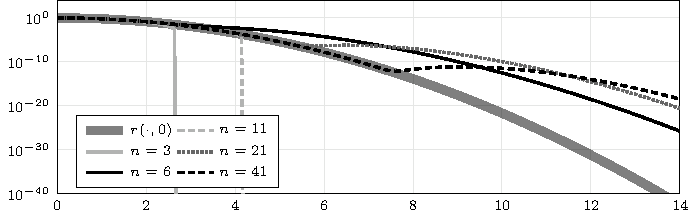
\includegraphics{Figures/fig_gaussian_truncation.pdf}}\label{fig:gaussian-truncation}
  \end{center}
  \caption{The Gaussian kernel~\eqref{eq:gaussian-kernel} with $u = 0$ and its
  truncated expansions in~\eqref{eq:gaussian-kernel-truncated}. For $n = 3$
  and $n = 11$ the truncated kernels become negative.}
\end{figure}

Define the truncated kernel
\begin{equation}
  \label{eq:gaussian-kernel-truncated} r_n (t, u) = \sum_{m = 0}^{n - 1}
  \psi_m (t) \psi_m (u)
\end{equation}
for any $n \in \N$. A few truncations are shown in 
Figure~\ref{fig:gaussian-truncation}. The truncated kernel converges to the
full Gaussian kernel $r$ pointwise on $\R \times \R$. The following
proposition shows that the convergence of~\eqref{eq:gaussian-kernel-truncated}
to $r$ is exponential in $\mathscr{L}_2 (\R \times \R, w_{\alpha} \otimes
w_{\alpha})$.

\begin{proposition}
  [Gaussian truncation]\label{prop:gaussian-truncation-error}Let $\alpha =
  \sqrt{\smash{[} b] 2 / 3}$. For every $n \in \N$ it holds that
  \[ \left( \int_{- \infty}^{\infty} \int_{- \infty}^{\infty} (r (t, u) - r_n
     (t, u))^2 w_{\alpha} (t) w_{\alpha} (u) \dif t \dif u \right)^{1 / 2} =
     \frac{1}{\sqrt{2}}  \hspace{0.17em} \frac{1}{3^n} . \]
\end{proposition}

\begin{proof}
  As in the proof of  Proposition~\ref{prop:matern-truncation-error}, we get
  \[ \int_{- \infty}^{\infty} \int_{- \infty}^{\infty} (r (t, u) - r_n (t,
     u))^2 w_{\alpha} (t) w_{\alpha} (u) \dif t \dif u = \sum_{m = n}^{\infty}
     \normstar{0}{\psi_m}_{\mathscr{L}_2 (\R, w_{\alpha})}^4 . \]
  By  Proposition~\ref{prop:gaussian-basis-L2},
  \[ \sum_{m = n}^{\infty} \normstar{0}{\psi_m}_{\mathscr{L}_2 (\R,
     w_{\alpha})}^4 = \sum_{m = n}^{\infty} \frac{4}{9^{m + 1}} = \frac{1}{2} 
     \hspace{0.17em} \frac{1}{9^n} . \]
  This completes the proof.
\end{proof}

\section{Conclusion}

In this article, we have demonstrated that  Theorem~\ref{thm:main-theorem} is
a simple and powerful tool for constructing orthonormal expansions of
translation-invariant kernels. In particular, using the Cholesky factor of the
Fourier transform of the kernel together with the Laguerre functions led to an
interesting decomposition of the RKHS of the Mat{\'e}rn kernel for
half-integer smoothness parameters in terms of a finite dimensional space and
a Hilbert space of functions vanishing at the origin. This might be deemed
unsatisfying, and a possible avenue to obtaining basis functions for
Mat{\'e}rns in a common space would be to investigate constructions based on
the symmetric square-root. The expansion for the Cauchy kernel was derived
from the Fourier duality with the Mat{\'e}rn kernel of smoothness $\alpha = 1
/ 2$. It remains an open problem to find a weighted $\mathscr{L}_2$ space in
which the Cauchy basis functions are orthogonal. For the Gaussian kernel, our
construction is a means to reproduce certain Mercer expansions that are
typically derived from Mehler's formula.

\section*{Acknowledgements}

FT was partially supported by the Wallenberg AI, Autonomous Systems and
Software Program (WASP) funded by the Knut and Alice Wallenberg Foundation,
and gratefully acknowledge financial support through funds from the Ministry
of Science, Research and Arts of the State of Baden-W{\"u}rttemberg.TK was
supported by the Academy of Finland postdoctoral researcher grant 338567
``Scalable, adaptive and reliable probabilistic integration''. Most of this
article was written while TK was visiting the University of T{\"u}bingen in
May 2022.

\begin{thebibliography}{10}
  \bibitem[1]{Adler1990}\tmtextsc{Adler, R.~J.} {\newblock}\tmtextit{An
  Introduction to Continuity, Extrema, and Related Topics for General Gaussian
  Processes}. {\newblock}No.~12 in Lecture Notes--Monograph Series. Institute
  of Mathematical Statistics, 1990.
  
  \bibitem[2]{AskeyWimp1984}\tmtextsc{Askey, R., and Wimp, J.}
  {\newblock}Associated Laguerre and Hermite polynomials.
  {\newblock}\tmtextit{Proceedings of the Royal Society of Edinburgh Section
  A: Mathematics 96}, 1--2 (1984), 15--37.
  
  \bibitem[3]{Bell2004}\tmtextsc{Bell, W.~W.} {\newblock}\tmtextit{Special
  Functions for Scientists and Engineers}. {\newblock}Courier Corporation,
  2004.
  
  \bibitem[4]{Christov1982}\tmtextsc{Christov, C.} {\newblock}A complete
  orthonormal system of functions in $L^2 (- \infty, \infty)$ space.
  {\newblock}\tmtextit{SIAM Journal on Applied Mathematics 42}, 6 (1982),
  1337--1344.
  
  \bibitem[5]{DickKuoSloan2013}\tmtextsc{Dick, J., Kuo, F.~Y., and Sloan,
  I.~H.} {\newblock}High-dimensional integration: The quasi-Monte Carlo way.
  {\newblock}\tmtextit{Acta Numerica 22} (2013), 133--288.
  
  \bibitem[6]{Erdelyi1954}\tmtextsc{Erd{\'e}lyi, A.}
  {\newblock}\tmtextit{Tables of Integral Transforms. Volume II}.
  {\newblock}McGraw-Hill, 1954.
  
  \bibitem[7]{FasshauerHickernell2012}\tmtextsc{Fasshauer, G., Hickernell, F.,
  and Wo{\'z}niakowski, H.} {\newblock}On dimension-independent rates of
  convergence for function approximation with Gaussian kernels.
  {\newblock}\tmtextit{SIAM Journal on Numerical Analysis 50}, 1 (2012),
  247--271.
  
  \bibitem[8]{FasshauerMcCourt2015}\tmtextsc{Fasshauer, G., and McCourt, M.}
  {\newblock}\tmtextit{Kernel-based Approximation Methods using MATLAB}.
  {\newblock}No.~19 in Interdisciplinary Mathematical Sciences. World
  Scientific Publishing, 2015.
  
  \bibitem[9]{FasshauerMcCourt2012}\tmtextsc{Fasshauer, G.~E., and McCourt,
  M.~J.} {\newblock}Stable evaluation of Gaussian radial basis function
  interpolants. {\newblock}\tmtextit{SIAM Journal on Scientific Computing 34},
  2 (2012), A737--A762.
  
  \bibitem[10]{Gnewuch2022}\tmtextsc{Gnewuch, M., Hefter, M., Hinrichs, A.,
  and Ritter, K.} {\newblock}Countable tensor products of Hermite spaces and
  spaces of Gaussian kernels. {\newblock}\tmtextit{Journal of Complexity 71}
  (2022), 101654.
  
  \bibitem[11]{Hawkins1989}\tmtextsc{Hawkins, D.~L.} {\newblock}Some practical
  problems in implementing a certain sieve estimator of the Gaussian mean
  function. {\newblock}\tmtextit{Communications in Statistics - Simulation and
  Computation 18}, 2 (1989), 481--500.
  
  \bibitem[12]{Higgins1977}\tmtextsc{Higgins, J.~R.}
  {\newblock}\tmtextit{Completeness and Basis Properties of Sets of Special
  Functions}. {\newblock}No.~72 in Cambridge Tracts in Mathematics. Cambridge
  University Press, 1977.
  
  \bibitem[13]{IrrgeherLeobacher2015}\tmtextsc{Irrgeher, C., and Leobacher,
  G.} {\newblock}High-dimensional integration on $\mathbb{R}^d$, weighted
  Hermite spaces, and orthogonal transforms. {\newblock}\tmtextit{Journal of
  Complexity 31}, 2 (2015), 174--205.
  
  \bibitem[14]{Karvonen2022}\tmtextsc{Karvonen, T.} {\newblock}Small sample
  spaces for Gaussian processes. {\newblock}\tmtextit{Bernoulli 29}, 2 (2023),
  875--900.
  
  \bibitem[15]{KimeldorfWahba1970}\tmtextsc{Kimeldorf, G.~S., and Wahba, G.}
  {\newblock}A correspondence between Bayesian estimation on stochastic
  processes and smoothing by splines. {\newblock}\tmtextit{The Annals of
  Mathematical Statistics 41}, 2 (1970), 495--502.
  
  \bibitem[16]{Kuo1975}\tmtextsc{Kuo, H.-H.} {\newblock}\tmtextit{Gaussian
  Measures in Banach Spaces}. {\newblock}No.~463 in Lecture Notes in
  Mathematics. Springer, 1975.
  
  \bibitem[17]{Minh2010}\tmtextsc{Minh, H.~Q.} {\newblock}Some properties of
  Gaussian reproducing kernel Hilbert spaces and their implications for
  function approximation and learning theory.
  {\newblock}\tmtextit{Constructive Approximation 32}, 2 (2010), 307--338.
  
  \bibitem[18]{NovakUllrich2018}\tmtextsc{Novak, E., Ullrich, M.,
  Wo{\'z}niakowski, H., and Zhang, S.} {\newblock}Reproducing kernels of
  Sobolev spaces on $\mathbb{R}^d$ and applications to embedding constants and
  tractability. {\newblock}\tmtextit{Analysis and Applications 16}, 5 (2018),
  693--715.
  
  \bibitem[19]{NovakWozniakowski2008}\tmtextsc{Novak, E., and
  Wo{\'z}niakowski, H.} {\newblock}\tmtextit{Tractability of Multivariate
  Problems. Volume I: Linear Information}. {\newblock}No.~6 in EMS Tracts in
  Mathematics. European Mathematical Society, 2008.
  
  \bibitem[20]{OwhadiScovel2017}\tmtextsc{Owhadi, H., and Scovel, C.}
  {\newblock}Separability of reproducing kernel spaces.
  {\newblock}\tmtextit{Proceedings of the American Mathematical Society 145},
  5 (2017), 2131--2138.
  
  \bibitem[21]{Paulsen2016}\tmtextsc{Paulsen, V.~I., and Raghupathi, M.}
  {\newblock}\tmtextit{An Introduction to the Theory of Reproducing Kernel
  Hilbert Spaces}. {\newblock}No.~152 in Cambridge Studies in Advanced
  Mathematics. Cambridge University Press, 2016.
  
  \bibitem[22]{RahimiRecht2007}\tmtextsc{Rahimi, A., and Recht, B.}
  {\newblock}Random features for large-scale kernel machines. {\newblock}In
  \tmtextit{Advances in Neural Information Processing Systems} (2007),
  vol.~20, pp.~1177--1184.
  
  \bibitem[23]{RasmussenWilliams2006}\tmtextsc{Rasmussen, C.~E., and Williams,
  C. K.~I.} {\newblock}\tmtextit{Gaussian Processes for Machine Learning}.
  {\newblock}Adaptive Computation and Machine Learning. MIT Press, 2006.
  
  \bibitem[24]{SolinSarkka2020}\tmtextsc{Solin, A., and S{\"a}rkk{\"a}, S.}
  {\newblock}Hilbert space methods for reduced-rank Gaussian process
  regression. {\newblock}\tmtextit{Statistics and Computing 30}, 2 (2020),
  419--446.
  
  \bibitem[25]{Stein1999}\tmtextsc{Stein, M.~L.}
  {\newblock}\tmtextit{Interpolation of Spatial Data: Some Theory for
  Kriging}. {\newblock}Springer Series in Statistics. Springer, 1999.
  
  \bibitem[26]{Steinwart2019}\tmtextsc{Steinwart, I.} {\newblock}Convergence
  types and rates in generic Karhunen-Lo{\`e}ve expansions with applications
  to sample path properties. {\newblock}\tmtextit{Potential Analysis 51}
  (2019), 361--395.
  
  \bibitem[27]{SteinwartScovel2012}\tmtextsc{Steinwart, I., and Scovel, C.}
  {\newblock}Mercer's theorem on general domains: On the interaction between
  measures, kernels, and RKHSs. {\newblock}\tmtextit{Constructive
  Approximation 35} (2012), 363--417.
  
  \bibitem[28]{Szego1939}\tmtextsc{Szeg{\H o}, G.}
  {\newblock}\tmtextit{Orthogonal Polynomials}. {\newblock}No.~23 in
  Colloquium Publications. American Mathematical Society, 1939.
  
  \bibitem[29]{VanTrees2001}\tmtextsc{Van~Trees, H.~L.}
  {\newblock}\tmtextit{Detection Estimation and Modulation Theory: Part I}.
  {\newblock}Wiley-Interscience, 2001.
  
  \bibitem[30]{Wendland2005}\tmtextsc{Wendland, H.}
  {\newblock}\tmtextit{Scattered Data Approximation}. {\newblock}No.~17 in
  Cambridge Monographs on Applied and Computational Mathematics. Cambridge
  University Press, 2005.
  
  \bibitem[31]{Wiener1949}\tmtextsc{Wiener, N.}
  {\newblock}\tmtextit{Extrapolation, Interpolation, and Smoothing of
  Stationary Time Series: With Engineering Applications}. {\newblock}MIT
  Press, 1949.
  
  \bibitem[32]{Xiu2010}\tmtextsc{Xiu, D.} {\newblock}\tmtextit{Numerical
  Methods for Stochastic Computations}. {\newblock}Princeton University Press,
  2010.
  
  \bibitem[33]{Zhu1998}\tmtextsc{Zhu, H., Williams, C. K.~I., Rohwer, R., and
  Morciniec, M.} {\newblock}Gaussian regression and optimal finite dimensional
  linear models. {\newblock}In \tmtextit{Neural Networks and Machine
  Learning}, C.~M. Bishop, Ed., vol.~168 of \tmtextit{NATO ASI Series. Series
  F: Computer and Systems Science}. Springer, 1998, pp.~167--184.
  
  \bibitem[34]{Zwickngaslc2009}\tmtextsc{Zwicknagl, B.} {\newblock}Power
  series kernels. {\newblock}\tmtextit{Constructive Approximation 29}, 1
  (2009), 61--84.
\end{thebibliography}

\end{document}
